\documentclass[11pt]{article}

% ---------------- Packages ----------------
\usepackage[a4paper,margin=1in]{geometry}
\usepackage{amsmath,amssymb,amsfonts}
\usepackage{mathtools}
\usepackage{bm}
\usepackage{booktabs}
\usepackage{array}
\usepackage{longtable}
\usepackage{tabularx}
\usepackage{enumitem}
\usepackage{graphicx}
\usepackage{caption}
\usepackage{subcaption}
\usepackage{float}
\usepackage{xcolor}
\usepackage[colorlinks=true,linkcolor=blue,citecolor=blue,urlcolor=blue]{hyperref}
\usepackage[activate={true,nocompatibility},final,tracking=true,kerning=true,spacing=true,factor=1100,stretch=10,shrink=10,expansion=false,protrusion=true]{microtype}
\usepackage{setspace}
\usepackage{titlesec}
\usepackage{fancyhdr}
\usepackage{footmisc}
\usepackage{parskip}
\usepackage{url}
\usepackage{xspace}
\usepackage{authblk}
\usepackage[numbers,sort&compress]{natbib}

\emergencystretch=3em
\graphicspath{{figures_v4/}}
\setlist[itemize]{leftmargin=1.6em,itemsep=0.25em,topsep=0.35em}
\setlist[enumerate]{leftmargin=1.6em,itemsep=0.25em,topsep=0.35em}
\titleformat{\section}{\Large\bfseries}{\thesection}{0.8em}{}
\titleformat{\subsection}{\large\bfseries}{\thesubsection}{0.8em}{}
\titleformat{\subsubsection}{\normalsize\bfseries\itshape}{\thesubsubsection}{0.6em}{}

\pagestyle{fancy}
\fancyhf{}
\fancyhead[L]{\small Mouse kidney spaceflight remodeling}
\fancyhead[R]{\small \thepage}
\renewcommand{\headrulewidth}{0.4pt}

\newcommand{\code}[1]{\texttt{#1}}
\newcommand{\pkg}[1]{\textsf{#1}}
\newcommand{\gene}[1]{\textit{#1}}
\newcommand{\RRRM}{RRRM-2\xspace}
\newcommand{\ISS}{ISS-T\xspace}
\newcommand{\LAR}{LAR\xspace}
\newcommand{\OSD}{OSDR\xspace}
\newcommand{\FDR}{FDR\xspace}

\title{\textbf{ISS-T, but not LAR, Aligns with a Recurrent ECM/Fibrosis and DCT/NCC-WNK Remodeling Axis in Mouse Kidney Spaceflight Transcriptomes}\\[0.35em]
\large RRRM-2 contrast analysis with OSD-513 recurrence and OSD-253 strain context}
\author{Ibrahim Shahid}
\affil{Independent research draft for mentor feedback\\Authorship/collaboration structure pending}
\date{Draft v4, May 2026}

\begin{document}
\maketitle

% =====================================================================
\section*{Executive summary for mentor feedback}

\noindent\textbf{Purpose of this draft.} This document is being shared to ask whether the claim hierarchy is biologically and statistically defensible, and whether the project is worth developing toward a preprint or journal submission.

\vspace{0.6em}
\small
\begin{tabularx}{\textwidth}{>{\bfseries}p{0.22\textwidth}X}
\toprule
Question & Can RRRM-2 kidney RNA-seq support an age- and arm-dependent spaceflight network-remodeling claim, and what biologically meaningful arm-specific signal is supported across OSDR cohorts? \\
\midrule
Datasets & RRRM-2 / OSD-771 is the factorial bridge cohort. OSD-513 is the primary external recurrence cohort. OSD-253 is used as a metadata-aware mechanism/context cohort, especially for C57BL/6J versus C3H/HeJ and original versus white-LED rerun ground controls. Tabula Muris Senis kidney is used as an external aging reference. \\
\midrule
Original claim status & RRRM-2 cannot support the original age-rewiring claim at primary module/pathway scale. Within-RRRM-2 control-aging vectors are too unstable for the planned contrast-of-contrasts interpretation. \\
\midrule
Main supported result & RRRM-2 ISS-T, not LAR, aligns with an independent OSD-513 kidney flight vector. The aligned direction is a matrix-high / DCT-low tubulointerstitial state: ECM/adhesion/proteolysis increases while DCT/NCC-WNK transport decreases. Mechanism scores support innate/TLR4 context, S1P/S1PR3, macrophage/inflammatory biology, adhesion/proteolysis, and tubular transport suppression. \\
\midrule
Mechanism boundary & OSD-253 suggests TLR4/innate association, not TLR4 requirement. The remodeling score is lower in C3H/HeJ at the point-estimate level, but strain-by-flight deltas are not significant and ECM/fibrosis/adhesion/proteolysis scores remain positive under the white-LED rerun control scenario. \\
\midrule
Feedback requested & Is this claim hierarchy biologically/statistically defensible? Is the cross-OSDR remodeling-axis story worth developing toward preprint/submission? What additional analysis, validation, or reframing would make the paper credible to space biology, kidney biology, or computational genomics reviewers? \\
\bottomrule
\end{tabularx}
\normalsize

\vspace{0.8em}
\noindent\textbf{Working claim structure.}
RRRM-2 cannot support the original age-rewiring claim. RRRM-2 ISS-T, not LAR, aligns with OSD-513. The aligned direction is matrix-high and DCT/NCC-WNK-low. OSD-253 suggests TLR4/innate association, not TLR4 requirement. WGCNA and sample-specific network methods are used as annotation and prioritization layers.

\clearpage

\section*{Plain-language summary}

\noindent
The original goal was to test whether spaceflight changes how mouse kidney aging networks behave. RRRM-2 is unusually useful for this because it includes young and old mice, flight and ground controls, and two mission arms. Each condition has only five mice, so the within-cohort aging-network direction is too noisy for the original age-rewiring claim. The supported result is arm-specific recurrence: the ISS terminal dissection arm of RRRM-2 points in the same pathway direction as an independent kidney spaceflight cohort, OSD-513. That shared direction looks like extracellular-matrix/fibrosis activation with distal tubule transport suppression. OSD-253 helps constrain mechanism: TLR4/innate biology tracks the score, while the strain comparison argues for a broader remodeling program. LIONESS and node2vec prioritize candidate local network-neighborhood contributors to that program.

\vspace{0.8em}

\begin{abstract}
\noindent
Spaceflight affects renal physiology, but the extent to which mouse kidney transcriptomes show age-dependent network remodeling remains unclear. We analyzed RRRM-2 (OSD-771), an age-by-arm-by-flight mouse kidney RNA-seq dataset, together with external OSDR cohorts using residualized expression, curated pathway scores, WGCNA modules, LIONESS sample-specific network summaries, node2vec local-neighborhood displacement, and cross-cohort contrast vectors. RRRM-2 could not support the original age-rewiring claim because control-aging vectors were unstable at primary module/pathway resolution. The strongest result emerged at the cross-cohort flight-vector level. RRRM-2 ISS-T aligned with OSD-513 at pathway scale (cosine 0.641; 95\% CI 0.351 to 0.814; directional permutation $p=0.127$), whereas RRRM-2 LAR anti-aligned with OSD-513 (cosine $-0.511$; CI $-0.726$ to $-0.231$; directional permutation $p=0.178$).

The recurring ISS-T/OSD-513 direction was extracellular-matrix/fibrosis-positive and DCT/NCC-WNK transport-negative. A state-space decomposition represented this as a matrix-high / DCT-low tubulointerstitial state, with the DCT component kept in its native biological direction. RRRM-2 ISS-T showed a strong positive state shift, whereas LAR did not. OSD-513 showed the same scalar direction, driven most strongly by DCT/NCC-WNK suppression. Mechanism scoring linked the state to ECM organization, TLR4/innate context, MMP/ADAM proteolysis, S1P/S1PR3 signaling, integrin/cell adhesion, macrophage/inflammatory signatures, and tubular transport suppression. OSD-253 constrained the mechanism: the remodeling program was attenuated at the point-estimate level in C3H/HeJ but remained positive, and several ECM/fibrosis/adhesion/proteolysis scores remained positive in C3H/HeJ. LIONESS/node2vec gene prioritization nominated exploratory local network-neighborhood contributors. These results support a reframed claim: ISS-T captures a recurrent kidney remodeling axis that is biologically coherent across OSDR cohorts and mechanistically testable in follow-up work.
\end{abstract}

\vspace{0.3em}
\noindent\textbf{Keywords:} spaceflight transcriptomics; mouse kidney; OSD-771; RRRM-2; OSD-513; OSD-253; LIONESS; node2vec; WGCNA; extracellular matrix; renal fibrosis; TLR4; S1P; distal convoluted tubule; NCC-WNK transport.

\clearpage
\tableofcontents
\clearpage

% =====================================================================
\section{Introduction}

\subsection{Spaceflight kidney biology is broader than kidney-stone risk}

Kidney risk has been part of human spaceflight medicine since early discussions of weightlessness-associated urolithiasis \citep{cockett1962astronautical}. Subsequent astronaut studies connected long-duration missions to altered calcium homeostasis, bone loss, and increased renal stone risk \citep{pietrzyk2007renal,smith2014men}. More recent space medicine has broadened this concern from stone formation alone to kidney remodeling, tubulopathy, solute handling, mitochondrial stress, vascular and interstitial changes, and multi-organ physiology \citep{siew2024cosmic,chouker2025impact,afshinnekoo2020fundamental}. Rodent spaceflight studies are central to this shift because kidney tissue can be collected directly and analyzed by histology, transcriptomics, and multi-omic profiling under controlled mission conditions \citep{daSilveira2020comprehensive,galazka2020rnaseq,finch2025strain}.

The biological question is not only whether spaceflight changes mean expression of individual genes. Kidney function depends on coordinated nephron-segment transport, immune activation, endothelial and interstitial remodeling, extracellular-matrix turnover, and stress-response programs. These processes can move together at module or pathway scale even when individual genes do not pass stringent differential-expression thresholds. Conversely, gene-level network metrics can look interesting without supporting a cohort-level biological program. The present study therefore treats network analysis as a multi-resolution problem: claims are strongest when pathway/module-scale direction, external recurrence, mechanism scoring, and exploratory gene prioritization point toward compatible biology.

\subsection{RRRM-2 defines a clean factorial contrast with limited per-cell precision}

NASA RRRM-2 (OSD-771) is a rare mouse kidney RNA-seq cohort with Age, mission Arm, and Environment Group represented in the same study. Young and old female C57BL/6NTac mice were sampled across flight, habitat ground-control, vivarium, and basal contexts, with ISS terminal dissection (ISS-T) and live animal return (LAR) arms. This design naturally invites a factorial question: does spaceflight amplify, dampen, or redirect age-associated kidney transcriptional network patterns differently in ISS-T and LAR?

For an arm $a\in\{\mathrm{ISS\mbox{-}T},\mathrm{LAR}\}$, the within-arm control-aging vector and flight-aging vector can be written as
\begin{equation}
A^a_{GC}=\bar{X}_{\mathrm{Old},a,GC}-\bar{X}_{\mathrm{Young},a,GC},
\qquad
A^a_{FLT}=\bar{X}_{\mathrm{Old},a,FLT}-\bar{X}_{\mathrm{Young},a,FLT}.
\end{equation}
The original scientific aim was to compare $A^a_{FLT}$ with $A^a_{GC}$. Projection of $A^a_{FLT}$ onto $A^a_{GC}$ would quantify aging-like amplification or dampening, while the residual component would quantify redirection. This is a clean conceptual formulation. The statistical difficulty is that $A^a_{GC}$ itself is estimated from only ten mice within each arm (five young GC and five old GC). A noisy control-aging direction makes downstream claims about amplification or redirection unstable.

This is a property of the estimand. High-dimensional contrast-of-contrasts are harder than simple flight-versus-ground comparisons, especially for network features whose uncertainty is already larger than mean-expression uncertainty. The analysis below therefore separates the original age-rewiring hypothesis from the cross-cohort flight-remodeling question that RRRM-2 can answer when paired with independent OSDR cohorts.

\subsection{Role of WGCNA and sample-specific network analyses}

Weighted gene co-expression network analysis (WGCNA) is useful for identifying co-expression modules, module eigengenes, hub genes, module-trait associations, and module preservation \citep{langfelder2008wgcna,langfelder2011preservation}. It is a sensible structural annotation method for kidney transcriptomics. However, standard WGCNA does not naturally test the factorial interaction at the heart of this project. A module eigengene can show age association, flight association, or arm association, but the method summarizes a module by its dominant variance axis. A smaller-variance interaction pattern within a module can be blurred by the eigengene. WGCNA is therefore valuable here as a module-scale biological layer, not as the sole primary inferential engine for age-dependent network rewiring.

Sample-specific network methods such as LIONESS estimate how each sample contributes to a shared network structure \citep{kuijjer2019estimating}. Embedding methods such as node2vec provide low-dimensional summaries of graph neighborhoods \citep{grover2016node2vec}. These approaches are useful for asking whether a gene's local network context changes, in addition to whether its mean expression changes. Given the cohort size and multiple-testing burden, this manuscript uses LIONESS/node2vec as exploratory local-neighborhood prioritization after establishing the pathway/module-level recurring direction.

\subsection{A cross-cohort contrast strategy}

The strategy in this manuscript is to pair RRRM-2 with external OSDR cohorts at the level of comparable pathway contrasts. RRRM-2 supplies the factorial bridge: it defines ISS-T and LAR flight directions under a controlled design. OSD-513 supplies an independent flight-vector recurrence test. OSD-253 supplies mechanistic and metadata-aware context because it includes C57BL/6J and C3H/HeJ mice and because C3H/HeJ has defective TLR4 signaling, making it useful for constraining TLR4-dependent interpretations. OSD-253 is analyzed as a mechanism-context cohort because original and rerun ground-control definitions trade off light history and sequencing/read-length comparability, and rodent spaceflight transcriptomes are known to be sensitive to sample collection and preservation factors \citep{galazka2020rnaseq,preserve2016}.

The resulting hierarchy is deliberately simple. First, RRRM-2 is tested for the original age-rewiring claim. Second, RRRM-2 arm-specific flight vectors are tested against OSD-513. Third, the aligned direction is decomposed into a matrix-high / DCT-low tubulointerstitial state. Fourth, OSD-253 is used to ask whether the state is TLR4-associated or TLR4-dependent. Fifth, WGCNA, LIONESS, and node2vec are used to annotate and prioritize genes within the pathway-level program.

% =====================================================================
\section{Methods}

\subsection{Datasets and metadata handling}

\subsubsection{RRRM-2 / OSD-771}

RRRM-2 (OSD-771) was the discovery and factorial bridge cohort. The analysis used kidney RNA-seq from female C57BL/6NTac mice in a design crossing Age (Young and Old), mission Arm (ISS-T and LAR), and Environment Group (FLT, Habitat Ground Control, Vivarium Control, Basal), with $n=5$ biological replicates per Age $\times$ Arm $\times$ Environment cell. ISS-T and LAR were treated as distinct mission-arm/recovery-context strata rather than as a simple duration contrast. Primary flight contrasts used FLT and Habitat Ground Control samples. Vivarium and Basal samples were retained for preprocessing context and metadata completeness but were not pooled into the primary FLT-versus-GC vectors.

\subsubsection{OSD-513}

OSD-513 was used as the primary external recurrence cohort because it contains a powered mouse kidney flight comparison with $n=9$ FLT and $n=9$ Habitat Ground Control samples, plus additional context samples. It is not identical to RRRM-2 in sex, mission, strain substrain, or metadata, so it was not pooled with RRRM-2 at raw-expression level. Instead, the OSD-513 flight-minus-ground pathway vector was compared to RRRM-2 arm-specific flight vectors.

\subsubsection{OSD-253}

OSD-253 was used as a mechanistic and metadata-aware context cohort. It contains C57BL/6J and C3H/HeJ samples and therefore provides an opportunity to ask whether an ISS-T-aligned remodeling score is attenuated in a TLR4-impaired strain background. However, OSD-253 also has control-definition complexity. Original ground controls are closer to the original sequencing context but have light-history mismatch, whereas 2021 white-LED rerun controls improve the light comparison but introduce read-length/library comparability concerns. Therefore, both scenarios were run, and OSD-253 was not treated as a single clean validation endpoint.

\subsubsection{External kidney aging reference}

Tabula Muris Senis kidney data were used to construct an independent mouse kidney aging axis \citep{tabula2020}. Female kidney single-cell profiles were aggregated to donor-level pseudobulk expression, and the primary external aging vector was defined as 18-month minus 3-month donor expression. This reference is useful because it prevents the small RRRM-2 GC aging direction from being the only definition of kidney aging, but it differs from RRRM-2 in age range, platform, and cell capture.

\subsection{Expression preprocessing and residualized matrix}

All primary RRRM-2 analyses used the residualized expression matrix and matched sample metadata generated by the project preprocessing pipeline. Upstream preprocessing included expression filtering, variance-stabilizing transformation, cell-type deconvolution, and residualization against technical and cellular-composition covariates. The purpose of residualization was to reduce the chance that apparent network or pathway shifts were driven only by changes in estimated kidney cell-type proportions. The residualized matrix was used for pathway scoring, module projection, and sample-specific node summaries.

External OSDR cohorts were processed with study-specific expression resources. Because OSDR studies differ in mission design, sequencing details, strain, sex, and metadata structure, external cohorts were compared at the level of within-study contrasts rather than by pooled sample-level modeling.

\subsection{Feature resolutions}

Four feature resolutions were used.

\textbf{Pathway resolution.} Curated kidney-relevant gene sets were scored per sample by averaging residualized expression across genes represented in the feature universe. The main pathway panel included DCT/NCC-WNK transport, ECM remodeling, fibrosis, apoptosis, oxidative stress, inflammation, calcium handling, lipid metabolism, and broad ion transport. DCT/NCC-WNK was designated as the primary tubular-transport feature because it is more mechanistically coherent than broad ion transport.

\textbf{Module resolution.} WGCNA module eigengenes from the existing module run were used as module-level features. WGCNA modules were used to annotate coherent gene programs and to ask whether pathway-scale effects map onto unsupervised co-expression architecture.

\textbf{Gene resolution.} Gene-level expression features were retained for sensitivity and exploratory analyses. Gene-level analyses were never used to override module/pathway stability because they carry larger multiple-testing and interpretability burdens.

\textbf{LIONESS-node and node2vec resolution.} LIONESS sample-specific networks were built on a shared topology/backbone. Per-sample incident edge strengths were aggregated to gene-level node-strength features. Separately, condition-level graph embeddings were aligned by Procrustes transformation and used to compute local-neighborhood displacement. These quantities were used only for exploratory candidate prioritization.

\subsection{Within-RRRM age-vector stability and decomposition}

For each arm and feature resolution, a control-aging vector was computed as Old GC minus Young GC:
\begin{equation}
A^a_{GC}=\bar{X}_{\mathrm{Old},a,GC}-\bar{X}_{\mathrm{Young},a,GC}.
\end{equation}
Bootstrap resampling was stratified by Age, Arm, and Environment Group. Each bootstrap replicate rebuilt $A^a_{GC}$ and computed its cosine similarity to the full-sample vector. Module and pathway resolutions were treated as primary biological resolutions. Gene and LIONESS-node resolutions were treated as secondary.

If a primary control-aging direction was stable, the planned decomposition would compare the flight-aging vector
\begin{equation}
A^a_{FLT}=\bar{X}_{\mathrm{Old},a,FLT}-\bar{X}_{\mathrm{Young},a,FLT}
\end{equation}
to $A^a_{GC}$. The projection coefficient
\begin{equation}
\beta^a = \frac{A^a_{FLT}\cdot A^a_{GC}}{\lVert A^a_{GC}\rVert^2}
\end{equation}
would quantify alignment along the control-aging axis: $\beta>1$ suggests amplification, $0<\beta<1$ suggests dampening, $\beta<0$ suggests reversal, and a large orthogonal residual suggests redirection. In the production run, primary module/pathway stability did not pass consistently, so this decomposition is not promoted as a main biological claim.

\subsection{Cross-OSDR flight-vector recurrence}

The arm-specific RRRM-2 flight vector at pathway resolution was computed as age-pooled FLT minus GC within each arm:
\begin{equation}
F^{\mathrm{RRRM2},a}=\bar{X}_{\mathrm{FLT},a}-\bar{X}_{\mathrm{GC},a}.
\end{equation}
For an external study $s$, the corresponding flight vector was
\begin{equation}
F^s=\bar{X}^s_{\mathrm{FLT}}-\bar{X}^s_{\mathrm{GC}}.
\end{equation}
Vectors were compared using cosine similarity over shared pathway features. External uncertainty was estimated by bootstrap resampling within FLT and GC strata. A label-permutation sensitivity was also added for each external study/scenario by shuffling FLT/GC labels within the external cohort while holding the RRRM-2 arm-specific reference vector fixed. Directional permutation $p$ values report the fraction of shuffled external contrasts with cosine at least as positive as the observed value for positive alignments, or at least as negative for anti-alignments. OSD-513 was interpreted under a recurrence boundary. OSD-253 was interpreted under a context-sensitivity boundary because of metadata and control-scenario caveats.

\subsection{Recurrent remodeling-axis construction}

A recurrent ISS-T remodeling axis was constructed from pathways that were concordant between RRRM-2 ISS-T and OSD-513. Let $u_p$ be the unit-normalized RRRM-2 ISS-T effect for pathway $p$ and $v_p$ the unit-normalized OSD-513 effect. The raw pathway weight was the mean directional contribution from the two cohorts. The final axis was oriented so ECM/fibrosis activity was positive and DCT/NCC-WNK transport suppression was negative. Pathways with discordant signs were excluded from the primary axis. Broad ion transport was retained only as a sensitivity feature when its direction was mixed.

For each sample $i$, a scalar remodeling score was computed as
\begin{equation}
S_i = \sum_{p\in P_{\mathrm{axis}}} z(X_{ip})w_p,
\end{equation}
where $z(X_{ip})$ is the standardized pathway activity and $w_p$ is the unit-normalized recurrent-axis weight. Higher $S_i$ indicates a sample that is more similar to the recurrent ISS-T/OSD-513 remodeling direction.

\subsection{Mechanism scoring}

Mechanism signatures were defined in the versioned mechanism gene-set configuration file. Signatures included TLR4/innate immune signaling, TGF-beta/EMT/fibrosis, ECM organization, integrin/cell adhesion, S1P/S1PR3 signaling, MMP/ADAM proteolysis, DCT/NCC-WNK transport, broad tubular transport, oxidative stress/NRF2, macrophage/inflammatory context, and preservation/sample-stress response. Signatures were assigned roles as outcome anchors, candidate upstream mechanisms, or candidate context signatures.

To reduce circularity, axis-defining genes were dropped from mechanism signatures where possible before scoring. Coverage reports recorded requested genes, matched genes, scored genes, axis-overlap removals, and dropped genes. Mechanism scores were then tested against the scalar remodeling score by Spearman correlation within RRRM-2, OSD-513, and OSD-253. RRRM-2 and OSD-513 flight-minus-ground effects were also computed for mechanism scores.

\subsection{Tubulointerstitial state-space analysis}

The recurrent remodeling axis was also represented as a two-dimensional tubulointerstitial state space. This step was designed to make the biology legible without sign-flipping the DCT/NCC-WNK component. For each sample, mechanism scores were standardized within each study/scenario context. The matrix component was defined as
\begin{equation}
M_i=\frac{z(\mathrm{ECM}_i)+z(\mathrm{Integrin/adhesion}_i)+z(\mathrm{MMP/ADAM}_i)}{3}.
\end{equation}
The DCT transport component was defined in its native direction:
\begin{equation}
T_i=z(\mathrm{DCT/NCC\mbox{-}WNK}_i),
\end{equation}
where higher $T_i$ means stronger DCT/NCC-WNK transport signature. The plotted state space uses $M_i$ on the x-axis and $T_i$ on the y-axis. The matrix-high / DCT-low remodeling direction is therefore rightward and downward. A scalar state score was defined separately as
\begin{equation}
R_i=M_i-T_i.
\end{equation}
Higher $R_i$ means higher ECM/adhesion/proteolysis activity and lower DCT/NCC-WNK transport.

Two context components were computed in parallel: an immune-context component, defined as the mean of TLR4/innate and macrophage/inflammation z-scores, and a preservation-stress component, defined as the preservation/sample-stress z-score. FLT-minus-GC effects were computed for RRRM-2 ISS-T and LAR, age-pooled and age-stratified; OSD-513 FLT versus habitat ground control; and OSD-253 C57BL/6J and C3H/HeJ under both original-GC and white-LED rerun control definitions.

RRRM-2 state-space scores were joined to existing deconvolution outputs for DCT, fibroblast, immune, endothelial, proximal tubule, and TAL/LOH proportions. Spearman correlations tested whether $M_i$, $T_i$, immune context, preservation stress, or $R_i$ tracked estimated cell proportions. A targeted renal gene panel was extracted from the residualized RRRM-2 expression matrix for ECM/adhesion/proteolysis genes, TLR/innate/macrophage genes, DCT/NCC-WNK transport genes, and tubular/metabolic/network-priority genes observed in earlier analyses. This panel was used for biological visualization, not as an additional genome-wide discovery test.

\subsection{OSD-253 TLR4 discriminator}

OSD-253 was analyzed under two control scenarios: original ground controls and 2021 white-LED rerun ground controls. For each scenario and score, bootstrap estimates were computed for the C57BL/6J flight effect, the C3H/HeJ flight effect, and the C3H-minus-C57 strain delta. Interpretive labels were assigned as follows. A score was labeled \code{tlr4\_supported} only if the C57BL/6J effect was positive, the C3H/HeJ effect was attenuated, and the strain delta supported attenuation. A score was labeled \code{tlr4\_associated} if the score tracked the remodeling axis but remained positive in C3H/HeJ without a strain delta. Otherwise, it was labeled \code{inconclusive}. These labels summarize the strain-discriminator result for downstream interpretation.

\subsection{Exploratory LIONESS/node2vec local-neighborhood prioritization}

For each gene $g$, node2vec local-neighborhood displacement was computed separately in ISS-T and LAR:
\begin{equation}
D_g^{ISS}=1-\cos(v^{ISS,FLT}_g,v^{ISS,GC}_g),
\qquad
D_g^{LAR}=1-\cos(v^{LAR,FLT}_g,v^{LAR,GC}_g).
\end{equation}
ISS-T-specific embedding displacement was
\begin{equation}
\mathrm{Spec}_g=z(D_g^{ISS})-z(D_g^{LAR}).
\end{equation}
LIONESS node-strength effects were computed as FLT-minus-GC node-strength differences within each arm:
\begin{equation}
N_g^{ISS}=\bar{N}_{g,ISS,FLT}-\bar{N}_{g,ISS,GC},
\qquad
N_g^{LAR}=\bar{N}_{g,LAR,FLT}-\bar{N}_{g,LAR,GC}.
\end{equation}
The exploratory composite score was
\begin{equation}
C_g=z(D_g^{ISS})-z(D_g^{LAR})+z(|N_g^{ISS}|)-z(|N_g^{LAR}|)+0.5z(\mathrm{OSD513\ support}_g).
\end{equation}
An optional silent-shifter score penalized genes with strong ISS-T differential expression:
\begin{equation}
C^{silent}_g=C_g-z(|\log FC_g^{ISS}|).
\end{equation}
These scores nominate local network-neighborhood contributors to the recurrent remodeling program and are reported as prioritization metrics rather than formal gene-level discovery tests.

\subsection{Gene-priority enrichment and sensitivity}

Reported top-k enrichment used proportional thresholds only: top 1\%, 2\%, 5\%, and 10\% of the phase-specific gene universe. These correspond to 25, 50, 125, and 250 genes in the 2,500-gene production universe, and 50, 100, 250, and 500 genes in the 5,000-gene sensitivity universe. Fisher exact tests used the phase-specific gene universe as background and were BH-corrected across mechanism signatures within each ranking-score/threshold family. Ranked-list enrichment used a Mann-Whitney approach comparing composite scores inside versus outside each mechanism signature, with BH correction across signatures within each ranking score.

\subsection{Multiple testing and uncertainty accounting}

Benjamini-Hochberg correction was applied within explicitly defined test families \citep{benjamini1995controlling}. For mechanism-score correlations, FDR correction was applied across all non-missing score-versus-remodeling Spearman tests across the three study/scenario contexts reported in the mechanism association table. For OSD-513 mechanism flight effects, FDR correction was applied across the mechanism signatures tested in the OSD-513 FLT-versus-GC contrast. For the OSD-253 strain discriminator, FDR correction was applied separately within each control scenario and within each endpoint family: C57BL/6J flight effect, C3H/HeJ flight effect, and C3H-minus-C57 strain delta. For the exploratory gene-priority layer, top-k Fisher tests were corrected separately for each ranking score and proportional top-k threshold across mechanism signatures; ranked-list tests were corrected separately for each ranking score across mechanism signatures. WGCNA module-overlap tests were corrected across tested modules. Bootstrap confidence intervals for vector alignment, stability, and OSD-253 score effects were interpreted as uncertainty intervals rather than multiple-testing-adjusted significance tests. Cross-OSDR label-permutation $p$ values were reported as contrast-level sensitivity statistics and were not pooled into the mechanism-score FDR families.

The bootstrap resampled biological samples within fixed analysis definitions. It therefore captures sampling variability under the chosen preprocessing, residualization model, gene sets, pathway panel, and cohort metadata rules. It does not propagate uncertainty from gene-set curation, cell-type deconvolution reference choice, residualization model selection, feature-universe choice, or pathway-selection decisions. Sensitivity analyses addressed part of this fixed-pipeline uncertainty by using both OSD-253 control scenarios, a 2,500-gene production network universe and 5,000-gene sensitivity universe, proportional top-k thresholds, and leave-one-pathway-out cosine diagnostics. These sensitivity analyses do not replace prospective validation.

\subsection{Statistical software and reproducibility}

Analyses were implemented as a reproducible Python/R pipeline with versioned configuration files, run manifests, and scripted figure generation. Differential-expression and RNA-seq preprocessing resources follow standard Bioconductor practices \citep{ritchie2015limma,love2014deseq2,robinson2010edger}. Repository-internal commands, run identifiers, and output paths are listed in the Data and code availability section rather than in the main Methods text.

% =====================================================================
\section{Results}

\subsection{RRRM-2 cannot resolve the original age-rewiring contrast at primary resolution}

RRRM-2 was designed well for a factorial question, but its per-cell sample size is small for estimating high-dimensional aging directions. Bootstrap stability of within-arm GC aging vectors showed that primary module/pathway control-aging directions were unstable in three of four arm-resolution settings (Table~\ref{tab:stability}). LAR module passed, and gene/LIONESS-node summaries passed as secondary resolutions.

\begin{table}[H]
\centering\small
\begin{tabular}{llrrrrc}
\toprule
Arm & Resolution & Full norm & Median cosine & Lower CI & Required lower & Passed \\
\midrule
ISS-T & pathway & 0.167 & 0.787 & 0.248 & 0.400 & no \\
ISS-T & module & 0.325 & 0.750 & 0.056 & 0.400 & no \\
ISS-T & gene & 10.152 & 0.746 & 0.545 & 0.200 & yes \\
ISS-T & LIONESS-node & 10.152 & 0.745 & 0.549 & 0.200 & yes \\
LAR & pathway & 0.221 & 0.890 & 0.345 & 0.400 & no \\
LAR & module & 0.353 & 0.774 & 0.493 & 0.400 & yes \\
LAR & gene & 9.687 & 0.742 & 0.563 & 0.200 & yes \\
LAR & LIONESS-node & 9.687 & 0.737 & 0.556 & 0.200 & yes \\
\bottomrule
\end{tabular}
\caption{\textbf{Bootstrap angular stability of RRRM-2 control-aging vectors.} Module and pathway are the primary biological resolutions. Gene and LIONESS-node are secondary exploratory resolutions.}
\label{tab:stability}
\end{table}

This result sets the scale of the manuscript. RRRM-2 provides an arm-stratified flight contrast that can be tested for recurrence in external OSDR cohorts. The secondary stability of gene and LIONESS-node features motivates exploratory local-neighborhood prioritization, while the pathway/module claim rests on cross-cohort flight-vector recurrence.

\begin{figure}[H]
\centering
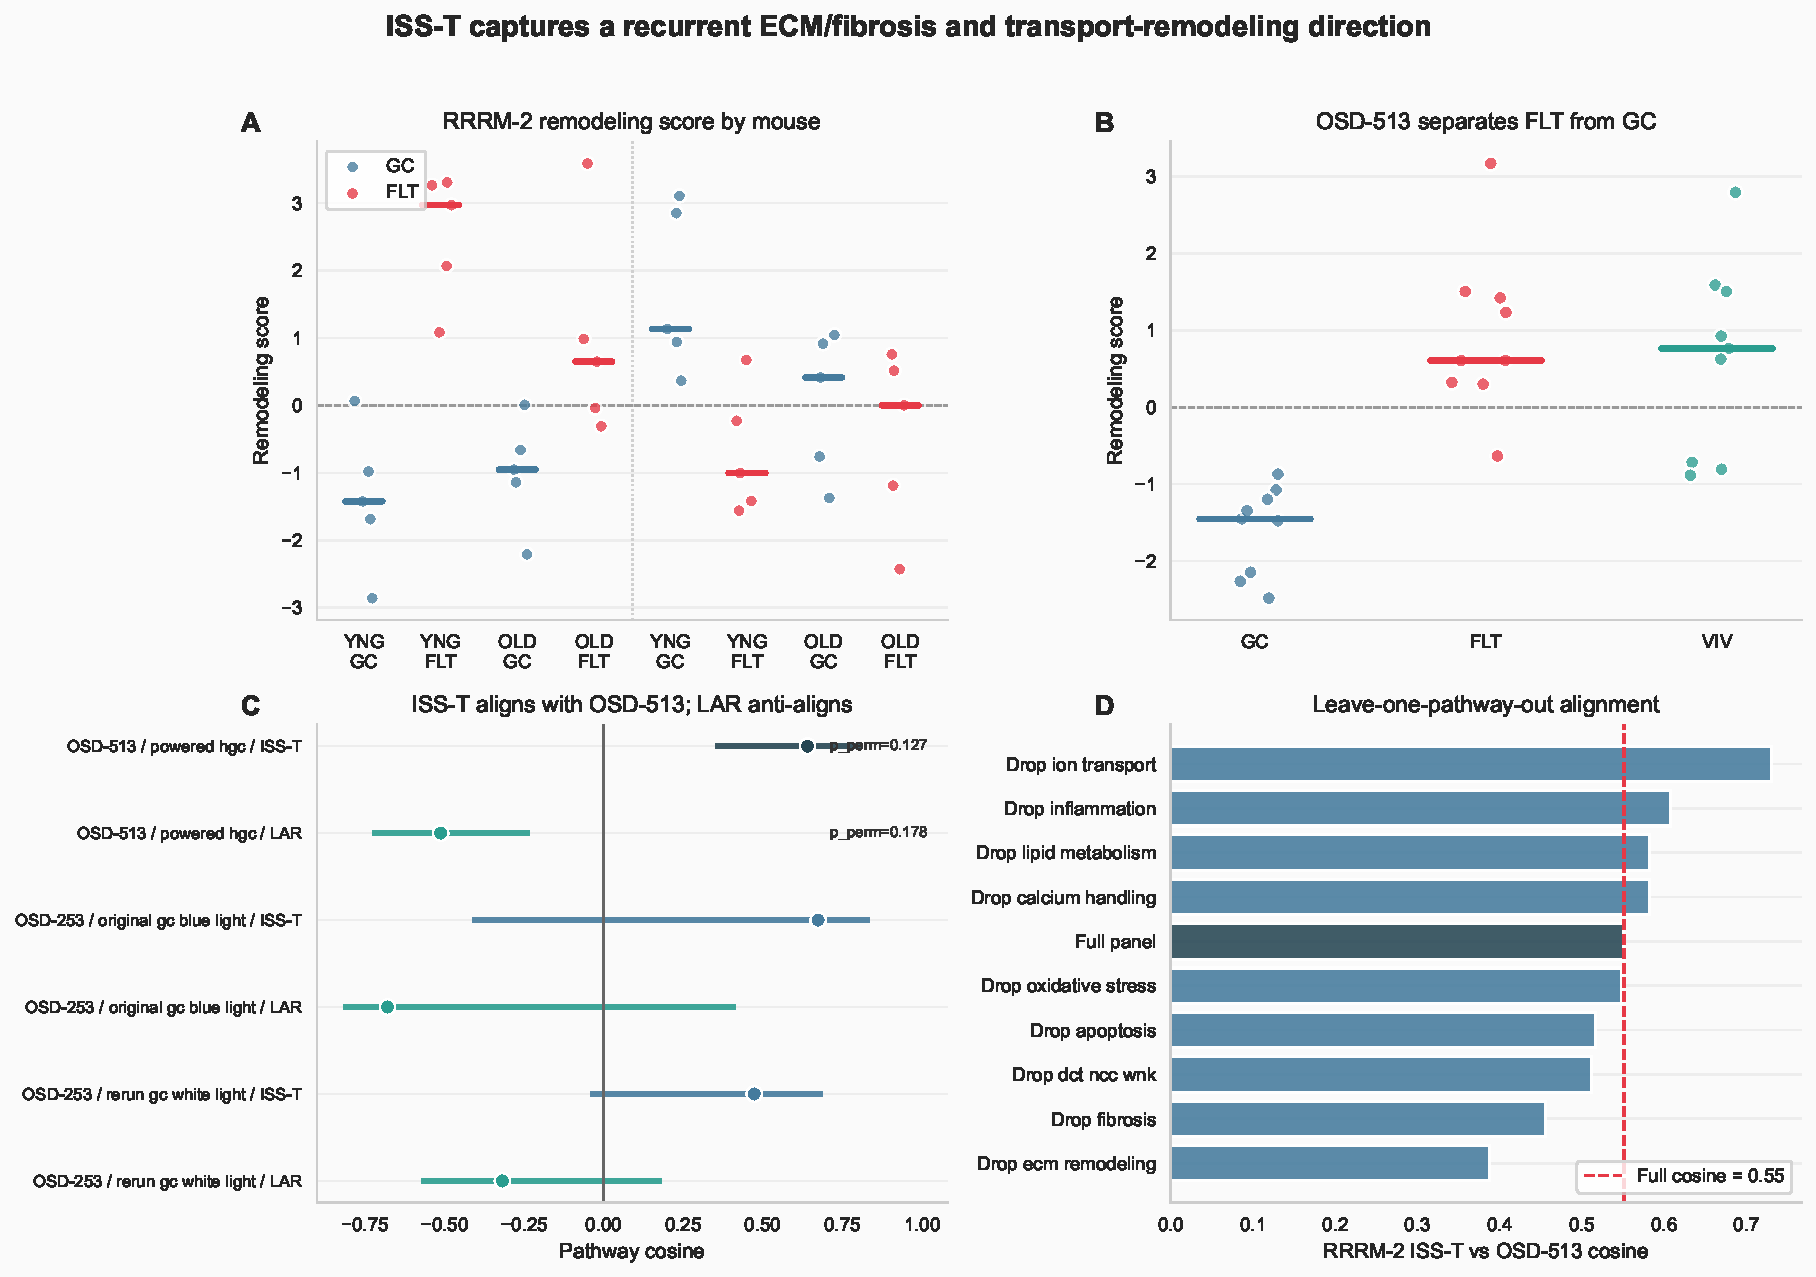
\includegraphics[width=\textwidth]{fig1_main_result_multipanel.pdf}
\caption{\textbf{Main result overview.} (A) RRRM-2 mouse-level remodeling scores by arm, age, and flight group. Points are individual mice; colored bars are group medians. (B) OSD-513 mouse-level separation on the same remodeling score. (C) Cross-OSDR pathway-vector alignment shows ISS-T alignment with OSD-513 and LAR anti-alignment. (D) Leave-one-pathway-out analysis shows that the alignment is not driven by a single pathway alone.}
\label{fig:mainresult}
\end{figure}

\subsection{ISS-T aligns with OSD-513; LAR anti-aligns}

The strongest positive result was arm-specific cross-OSDR alignment at pathway resolution. The RRRM-2 ISS-T flight vector aligned with the OSD-513 flight vector with cosine 0.641 and bootstrap 95\% CI 0.351 to 0.814. In the label-permutation sensitivity, the OSD-513 ISS-T cosine was above the null median near zero but did not reach a 0.05 directional permutation threshold ($p_{\mathrm{perm}}=0.127$). The RRRM-2 LAR vector was anti-aligned with OSD-513, with cosine $-0.511$, CI $-0.726$ to $-0.231$, and directional permutation $p=0.178$ (Table~\ref{tab:crossosdr}; Figure~\ref{fig:alignment}). OSD-253 C57BL/6J comparisons had positive ISS-T point estimates under both control definitions but wide confidence intervals crossing zero, so OSD-253 was carried forward as mechanism/context rather than recurrence evidence.

\begin{table}[H]
\centering\small
\resizebox{\textwidth}{!}{%
\begin{tabular}{lllrrrrrcc}
\toprule
Study & Scenario & Arm & Point & Median & Lower CI & Upper CI & $p_{\mathrm{perm}}$ & Boundary & Claimable \\
\midrule
OSD-513 & powered HGC & ISS-T & 0.641 & 0.625 & 0.351 & 0.814 & 0.127 & recurrence & yes \\
OSD-513 & powered HGC & LAR & -0.511 & -0.498 & -0.726 & -0.231 & 0.178 & recurrence & no \\
OSD-253 & original GC blue light & ISS-T & 0.674 & 0.602 & -0.411 & 0.836 & 0.141 & context & no \\
OSD-253 & original GC blue light & LAR & -0.679 & -0.608 & -0.816 & 0.415 & 0.125 & context & no \\
OSD-253 & rerun GC white light & ISS-T & 0.474 & 0.470 & -0.040 & 0.688 & 0.269 & context & no \\
OSD-253 & rerun GC white light & LAR & -0.318 & -0.309 & -0.572 & 0.183 & 0.344 & context & no \\
\bottomrule
\end{tabular}
}
\caption{\textbf{Cross-OSDR pathway-vector alignment.} OSD-513 is interpreted as directional recurrence. OSD-253 is interpreted as context sensitivity because of control-scenario caveats. $p_{\mathrm{perm}}$ is the directional external-label permutation sensitivity with the RRRM-2 reference vector held fixed.}
\label{tab:crossosdr}
\end{table}

\begin{figure}[H]
\centering
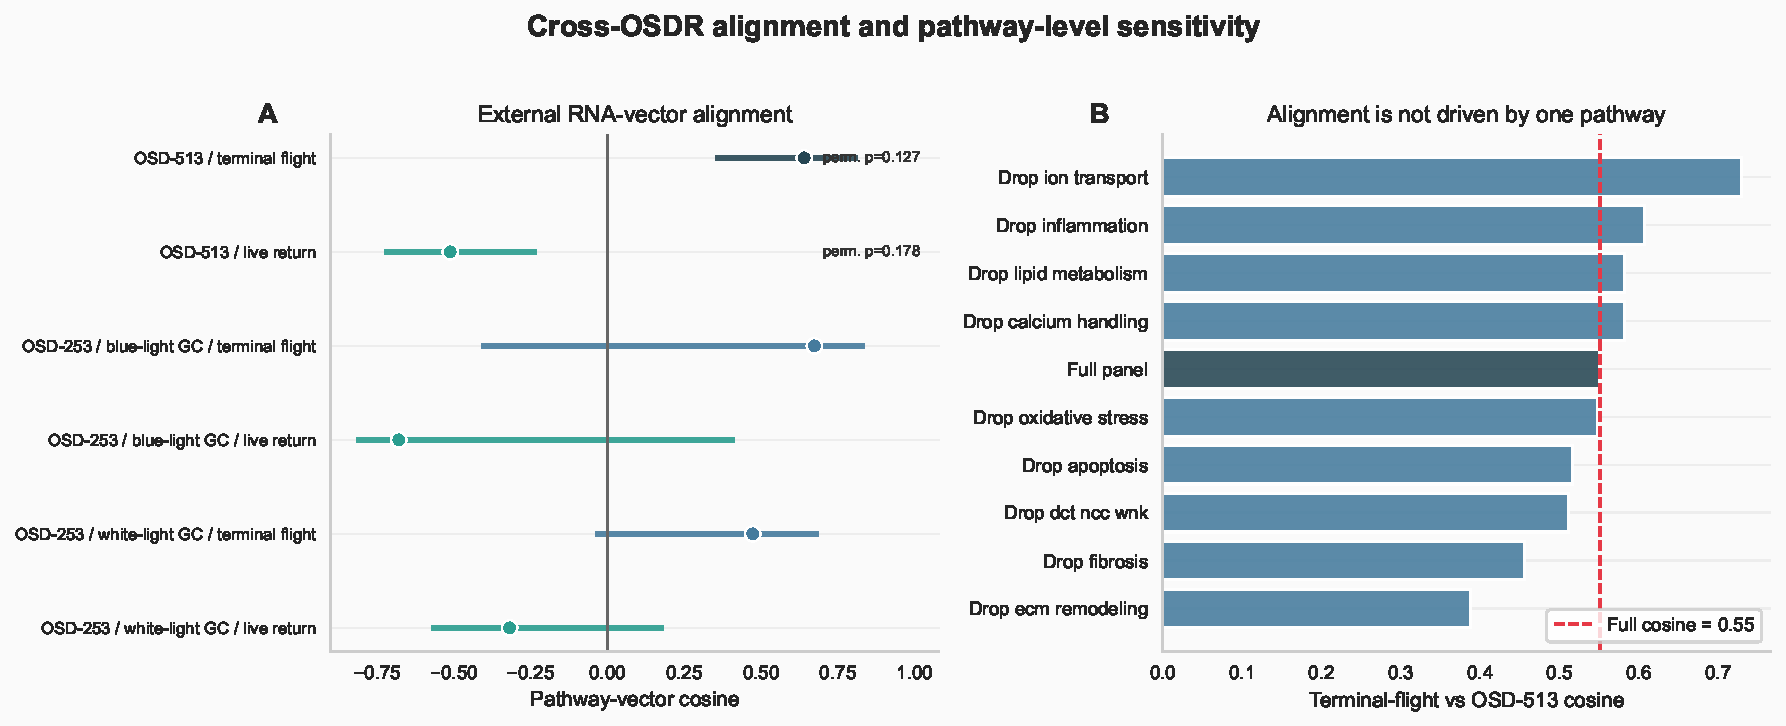
\includegraphics[width=\textwidth]{fig4_cross_alignment_leave_one_out.pdf}
\caption{\textbf{Cross-OSDR alignment and leave-one-pathway-out sensitivity.} (A) RRRM-2 arm-specific flight vectors compared with external OSDR pathway vectors. ISS-T aligns with OSD-513, whereas LAR anti-aligns; OSD-513 labels show directional external-label permutation $p$ values. (B) Leave-one-pathway-out cosines show that the RRRM-2 ISS-T/OSD-513 alignment is distributed across the pathway panel rather than fully dependent on a single component.}
\label{fig:alignment}
\end{figure}

The arm-specific sign pattern is the key biological finding. The terminal-flight arm captures a recurring flight-associated kidney remodeling direction. The return/recovery arm points in the opposite direction relative to OSD-513, especially for ECM/fibrosis features. This distinction is consistent with attenuation or reversal after return, while still leaving recovery timing and collection context as linked explanations.

\subsection{The recurrent axis is ECM/fibrosis-positive and DCT/NCC-WNK-negative}

Pathway-level decomposition identified the features that define the recurring ISS-T/OSD-513 direction. Concordant positive pathways were ECM remodeling, fibrosis, apoptosis, and oxidative stress. DCT/NCC-WNK transport was concordantly negative and therefore received a negative weight. Calcium handling, inflammation, broad ion transport, and lipid metabolism were excluded from the primary axis because they were discordant or mixed. Broad ion transport was retained as sensitivity only. The sample-level pathway scores show the same biological direction: ECM organization increases and DCT/NCC-WNK transport decreases most clearly in the RRRM-2 ISS-T and OSD-513 flight comparisons (Figure~\ref{fig:pathwayscores}).

\begin{figure}[H]
\centering
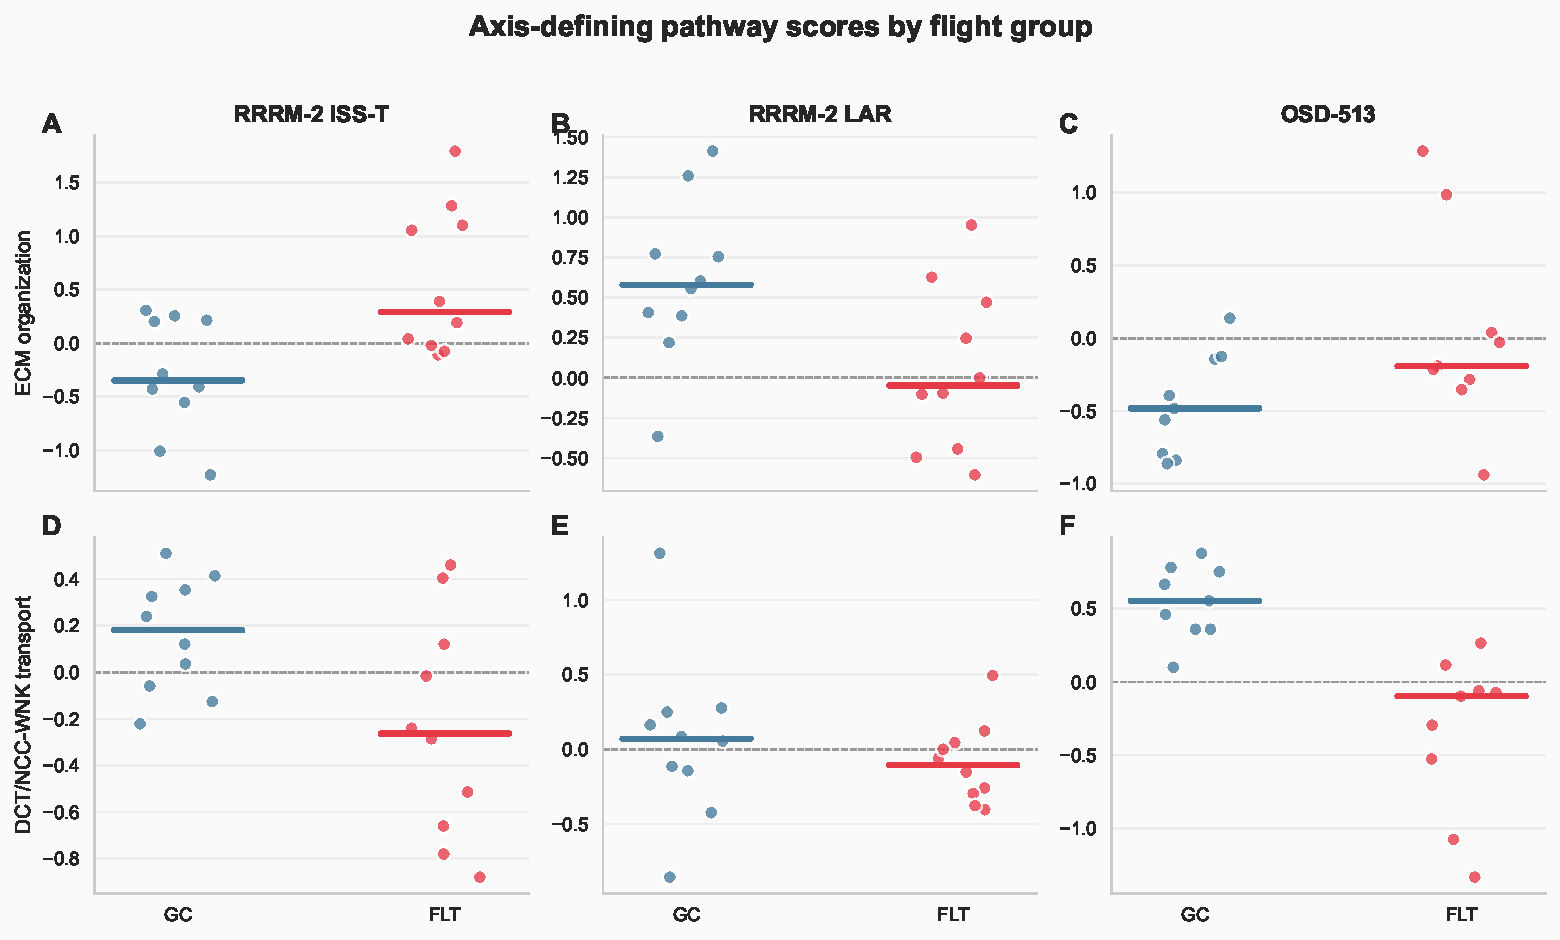
\includegraphics[width=\textwidth]{fig3_pathway_scores_by_flight.pdf}
\caption{\textbf{Axis-defining pathway scores by flight group.} Points are individual mice, and colored bars show medians. ECM organization increases and DCT/NCC-WNK transport decreases in the aligned RRRM-2 ISS-T and OSD-513 flight contexts.}
\label{fig:pathwayscores}
\end{figure}

\begin{table}[H]
\centering\small
\begin{tabular}{lrrrc}
\toprule
Pathway & RRRM-2 ISS-T effect & OSD-513 effect & Axis weight & Primary axis \\
\midrule
ECM remodeling & 0.949 & 0.801 & 0.622 & yes \\
Fibrosis & 0.764 & 0.652 & 0.504 & yes \\
DCT/NCC-WNK & -0.398 & -0.889 & -0.452 & yes \\
Apoptosis & 0.674 & 0.386 & 0.378 & yes \\
Oxidative stress & 0.198 & 0.104 & 0.108 & yes \\
Inflammation & 0.561 & -0.092 & 0.000 & no \\
Ion transport & 0.329 & -0.762 & 0.000 & sensitivity \\
Lipid metabolism & -0.320 & 0.156 & 0.000 & no \\
Calcium handling & 0.003 & -0.550 & 0.000 & no \\
\bottomrule
\end{tabular}
\caption{\textbf{Pathway construction of the recurrent ISS-T remodeling axis.} Effects are pathway-scale FLT-minus-GC contrasts. The final axis is oriented so ECM/fibrosis is positive and DCT/NCC-WNK suppression is negative.}
\label{tab:axisweights}
\end{table}

This axis provides the biological language for the rest of the manuscript: an ECM/fibrosis-positive and DCT/NCC-WNK-negative remodeling score that recurs between RRRM-2 ISS-T and OSD-513.

\subsection{A matrix-high / DCT-low tubulointerstitial state emerges across cohort context}

The recurrent axis can be read more directly as a two-dimensional tissue-state shift. The matrix component summarizes ECM organization, integrin/cell adhesion, and MMP/ADAM proteolysis. The DCT transport component is kept in its native biological direction, so higher values mean stronger DCT/NCC-WNK transport. The remodeling direction is therefore rightward and downward in state space, and the scalar \code{matrix\_minus\_dct} is defined as matrix component minus DCT transport component (Figure~\ref{fig:statespace}).

\begin{figure}[H]
\centering
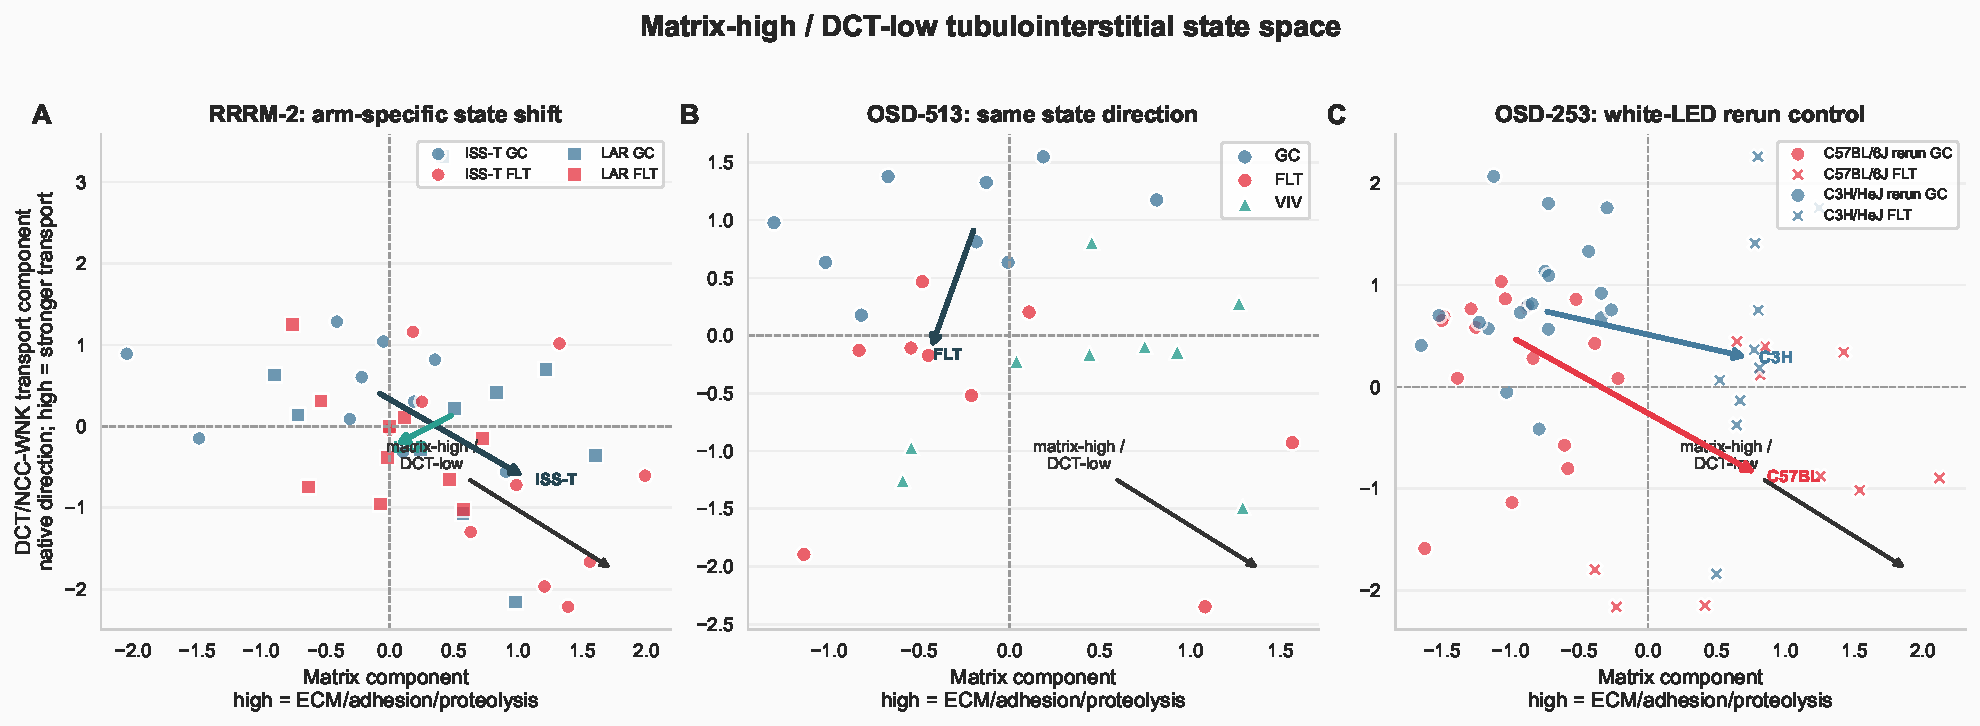
\includegraphics[width=\textwidth]{fig8_tubulointerstitial_state_space.pdf}
\caption{\textbf{Matrix-high / DCT-low tubulointerstitial state space.} The x-axis is the matrix component, where higher values indicate higher ECM/adhesion/proteolysis activity. The y-axis is the DCT/NCC-WNK transport component in native direction, where higher values indicate stronger DCT transport signature. The remodeling direction is rightward and downward. Points are individual mice. Arrows connect group medians from control to flight within the plotted context.}
\label{fig:statespace}
\end{figure}

The state-space effects sharpen the biological interpretation (Figure~\ref{fig:stateeffects}). RRRM-2 ISS-T showed a positive matrix shift (FLT-minus-GC effect $=1.25$, $q=0.0158$), a negative DCT transport shift ($-1.00$, $q=0.102$), and a strong positive matrix-minus-DCT state shift ($2.25$, $q=0.0163$). Immune-context and preservation-stress components were also higher in ISS-T flight ($1.16$, $q=0.0012$; $1.06$, $q=0.0310$). RRRM-2 LAR did not show the same state shift: matrix-minus-DCT was near zero ($-0.11$, $q=0.904$).

OSD-513 was directionally consistent at the scalar state level, with matrix-minus-DCT increasing in flight ($1.81$, $q=0.0310$). This OSD-513 state shift was driven most strongly by DCT/NCC-WNK suppression ($-1.57$, $q=0.0082$), while the matrix component was positive but not significant ($0.25$, $q=0.627$). This distinction matters: OSD-513 supports the same matrix-high/DCT-low direction, but it does not independently reproduce every component with equal strength. The OSD-513 label-permutation caveat remains part of the interpretation.

Under the OSD-253 white-LED rerun control scenario, both strains moved toward the matrix-high/DCT-low state. C57BL/6J showed a strong scalar effect ($2.68$, $q=2.3\times10^{-4}$) with matrix increase ($1.64$, $q=8.7\times10^{-4}$) and DCT decrease ($-1.04$, $q=0.072$). C3H/HeJ also showed a positive scalar effect ($1.82$, $q=0.0031$) and matrix increase ($1.51$, $q=3.1\times10^{-6}$), while its DCT component was only weakly negative ($-0.31$, $q=0.612$). Under the original-GC scenario, the scalar effects were weaker (C57BL/6J $0.79$, $q=0.229$; C3H/HeJ $-0.29$, $q=0.633$), reinforcing that OSD-253 is sensitive to control definition.

\begin{figure}[H]
\centering
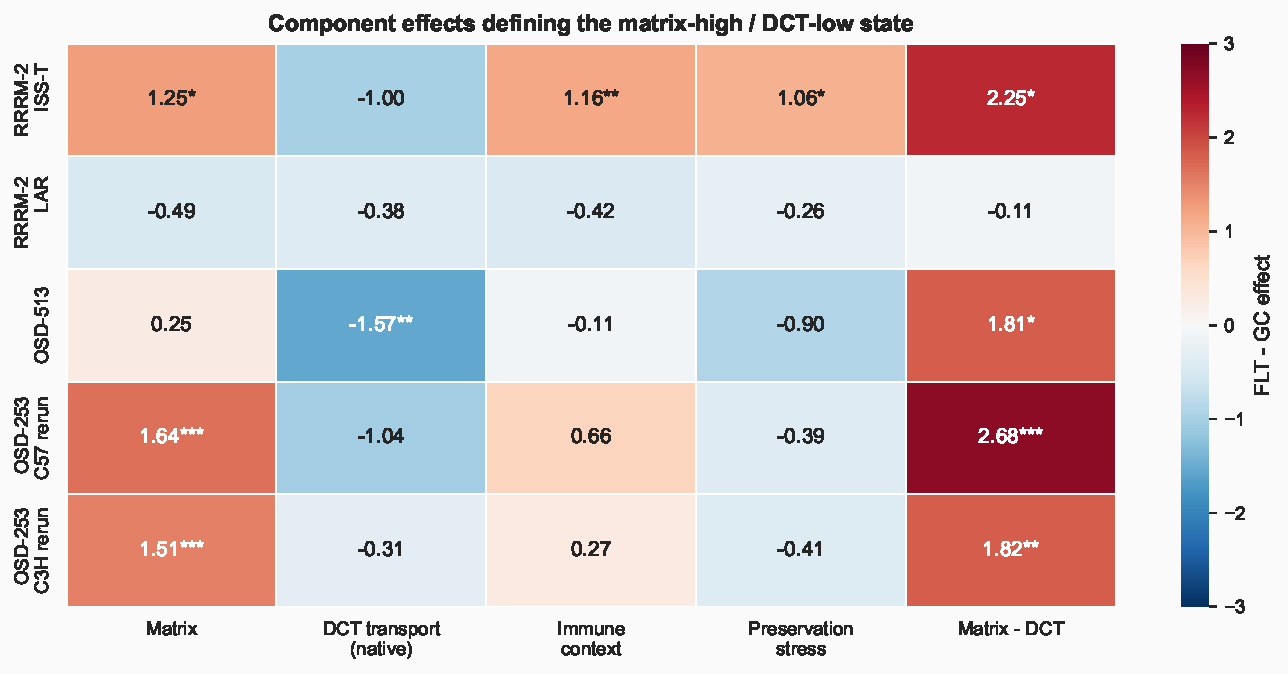
\includegraphics[width=\textwidth]{fig11_state_component_effects.pdf}
\caption{\textbf{Component effects defining the matrix-high / DCT-low state.} Values are FLT-minus-GC effects in standardized component units. Asterisks indicate BH-adjusted thresholds within the component-effect table. DCT transport is shown in native direction, so negative values indicate lower DCT/NCC-WNK transport signature in flight.}
\label{fig:stateeffects}
\end{figure}

RRRM-2 deconvolution estimates did not materially track the state components (Figure~\ref{fig:deconvoverlay}). All 80 RRRM-2 samples joined to the deconvolution table. Across tested state-component/cell-proportion pairs, the largest absolute Spearman correlation was small ($|\rho|=0.120$ for matrix component versus CLR fibroblast estimate), and all BH-adjusted $q$ values were approximately 0.99. Within the available deconvolution model, the matrix-high/DCT-low state is therefore not simply a readout of estimated DCT or fibroblast fraction.

\begin{figure}[H]
\centering
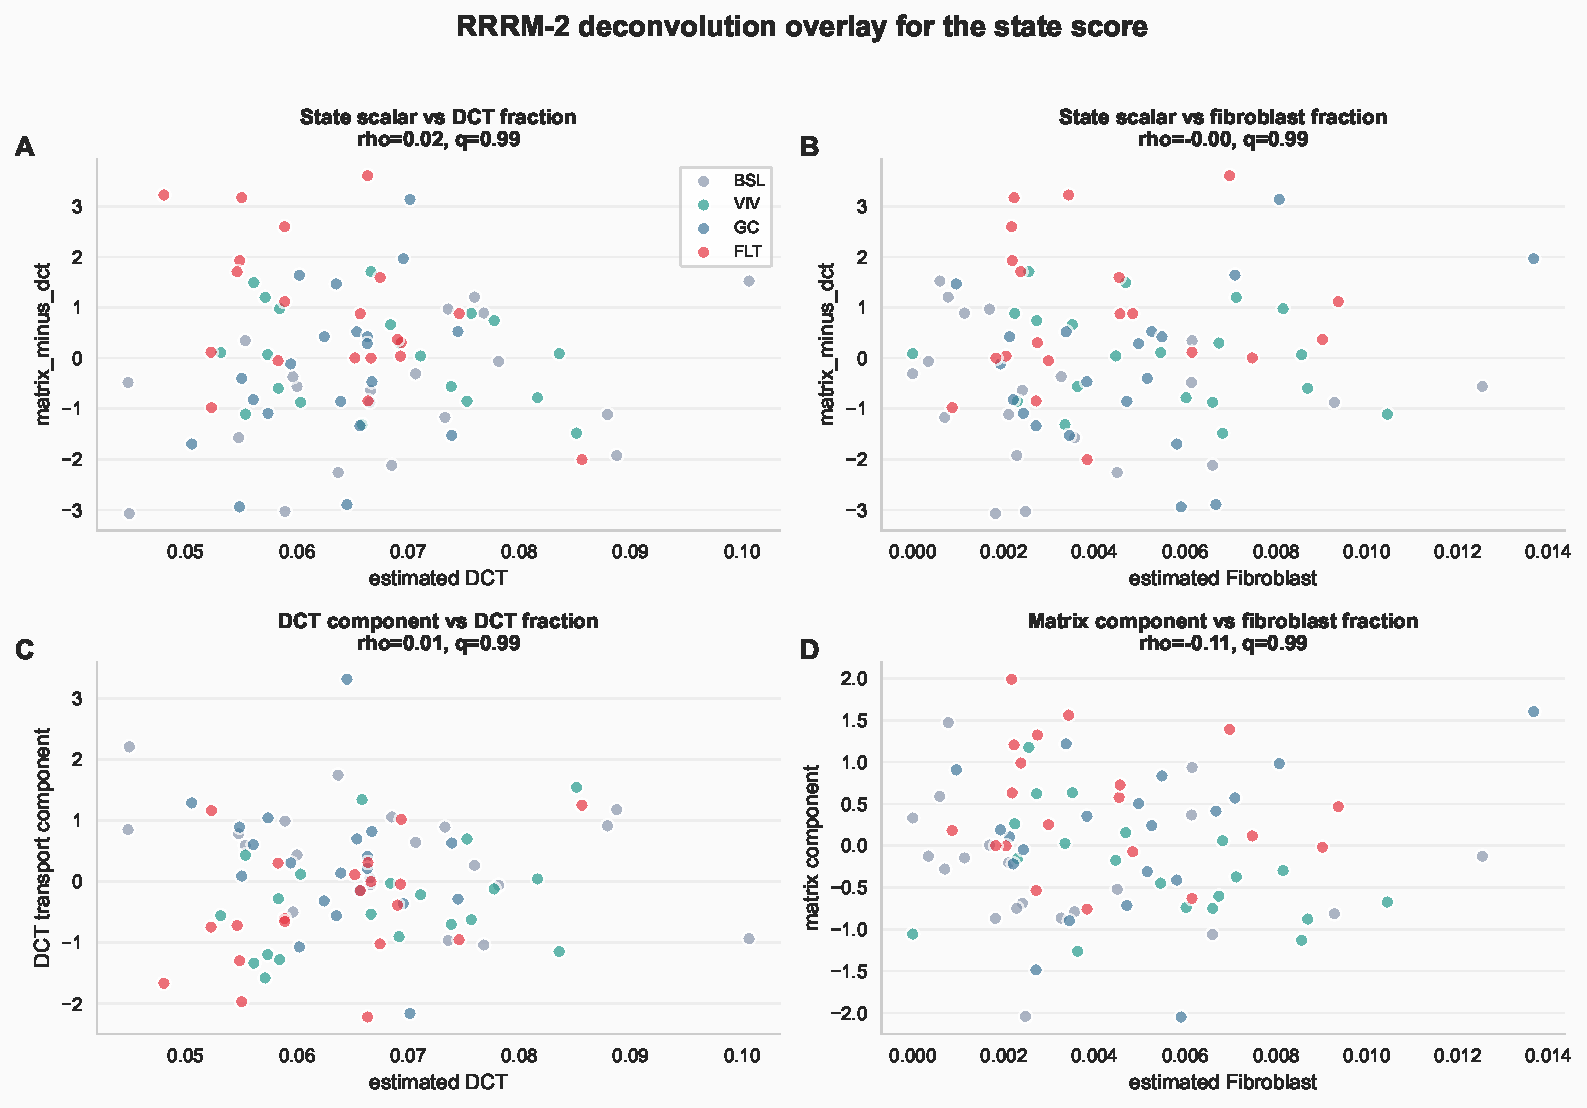
\includegraphics[width=\textwidth]{fig9_rrrm2_deconvolution_overlay.pdf}
\caption{\textbf{RRRM-2 deconvolution overlay for the tubulointerstitial state.} Points are individual RRRM-2 mice. The scalar state score and its components show little correlation with estimated DCT or fibroblast proportions, suggesting that the state-space signal is not explained by these deconvolution estimates alone.}
\label{fig:deconvoverlay}
\end{figure}

Finally, targeted residualized-expression visualization placed familiar renal genes inside the state interpretation (Figure~\ref{fig:renalpanel}). The panel includes 53 scored genes across ECM/adhesion/proteolysis, TLR/innate/macrophage, DCT/NCC-WNK transport, and tubular/metabolic-priority classes. This is a biological annotation display rather than an additional discovery test, but it is useful for seeing that the state-space result is carried by recognizable renal-remodeling and tubular-transport genes.

\begin{figure}[H]
\centering
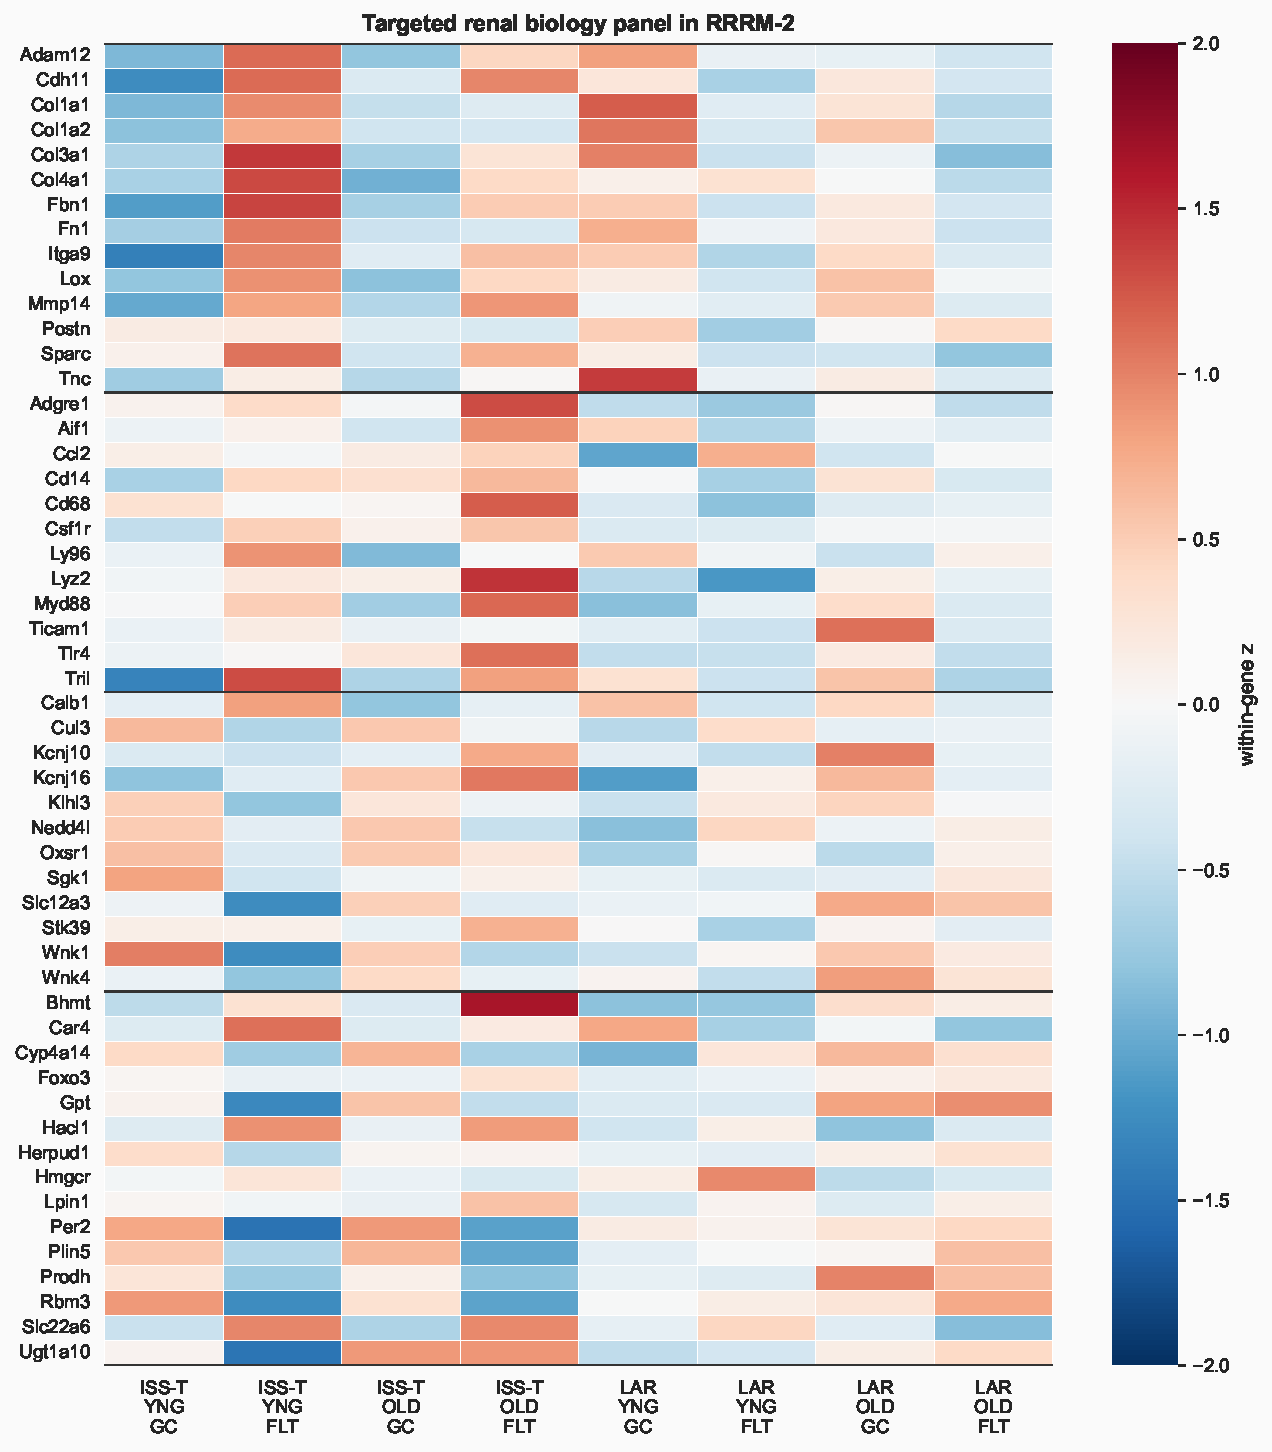
\includegraphics[width=0.95\textwidth]{fig10_targeted_renal_gene_heatmap.pdf}
\caption{\textbf{Targeted renal biology panel in RRRM-2.} Values are group-mean, within-gene z-scores from residualized expression. Rows are grouped by biology class: ECM/adhesion/proteolysis, TLR/innate/macrophage, DCT/NCC-WNK transport, and tubular/metabolic-priority genes.}
\label{fig:renalpanel}
\end{figure}

\subsection{Mechanism scores nominate ECM, innate, adhesion, S1P, and DCT programs}

Mechanism scoring asked which candidate upstream or contextual programs track the scalar remodeling score. In RRRM-2, the remodeling score correlated strongly with ECM organization ($\rho=0.644$, $q=7.4\times10^{-10}$), DCT/NCC-WNK transport suppression ($\rho=-0.560$, $q=3.1\times10^{-7}$), TLR4/innate signaling ($\rho=0.488$, $q=1.8\times10^{-5}$), MMP/ADAM proteolysis ($\rho=0.478$, $q=2.6\times10^{-5}$), S1P/S1PR3 signaling ($\rho=0.451$, $q=8.2\times10^{-5}$), and integrin/cell adhesion ($\rho=0.374$, $q=1.5\times10^{-3}$). OSD-513 reproduced the ECM-positive and DCT-negative relationship: ECM organization correlated with the remodeling score ($\rho=0.745$, $q=2.7\times10^{-5}$), and DCT/NCC-WNK transport correlated negatively ($\rho=-0.676$, $q=2.8\times10^{-4}$). OSD-253, across all samples, showed strong associations of the remodeling score with TLR4/innate signaling, ECM organization, macrophage/inflammatory context, DCT/NCC-WNK suppression, and S1P/S1PR3 (Figure~\ref{fig:mechheat}).

\begin{figure}[H]
\centering
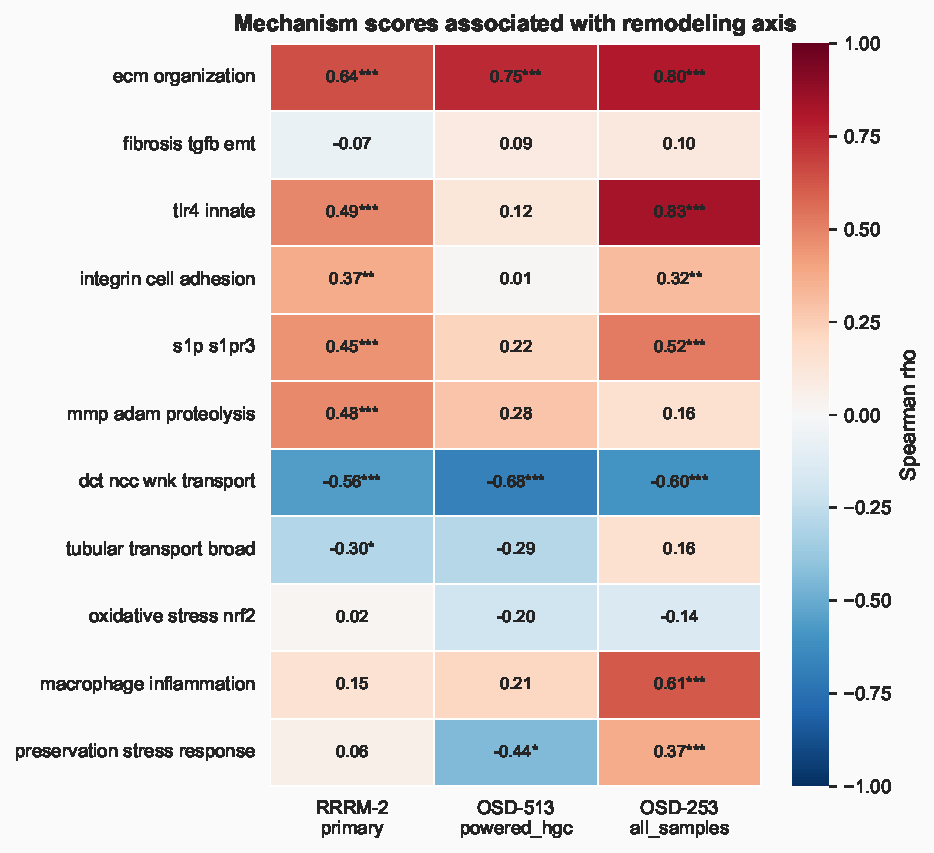
\includegraphics[width=0.82\textwidth]{fig6_mechanism_score_heatmap.pdf}
\caption{\textbf{Mechanism-score associations with the recurrent remodeling score.} Color indicates Spearman correlation between each mechanism score and the scalar remodeling score. Asterisks mark BH-adjusted $q<0.05$ within the association table. RRRM-2 and OSD-513 both show ECM-positive and DCT/NCC-WNK-negative structure. OSD-253 shows strong TLR4/innate, ECM, macrophage/inflammation, and transport relationships across its broader sample set.}
\label{fig:mechheat}
\end{figure}

The mechanism pattern is biologically plausible. TLR4 signaling is implicated in renal inflammation and fibrosis, and TLR4-mutant mice have been reported to be protected from chronic kidney disease progression and renal fibrosis \citep{souza2015tlr4}. TRIL is a co-receptor associated with TLR3/TLR4 signaling and cytokine production \citep{carpenter2009tril,wochal2014tril,carpenter2011tril}. Cadherin-11 has a recognized role in tissue fibrosis and fibroblast-like cell adhesion \citep{chavula2022cadherin}. Integrins and MMP/ADAM proteases are core mediators of cell-matrix adhesion and matrix turnover. Sphingosine-1-phosphate signaling, including S1PR3-centered biology, has been linked to kidney injury, inflammation, and fibrotic remodeling in several contexts \citep{s1p2017,s1p2020}. The DCT/NCC-WNK direction is also coherent with distal nephron transport regulation, where WNK-SPAK/OSR1-NCC signaling governs sodium-chloride cotransport and potassium-sensitive distal nephron physiology \citep{castaneda2024dct,ge2016wnk}.

The mechanism scores place the recurrent remodeling direction in a molecular neighborhood involving ECM deposition, adhesion/proteolysis, innate immune signaling, S1P biology, macrophage/inflammatory context, and tubular transport suppression. This supports a mechanism-prioritization model in which multiple upstream and downstream programs are carried forward for targeted validation.

\subsection{OSD-253 points to TLR4/innate association rather than TLR4 requirement}

OSD-253 was used as the immediate mechanistic discriminator because C3H/HeJ mice have impaired TLR4 signaling. A strict TLR4-dependent model predicts attenuation of the remodeling score in C3H/HeJ relative to C57BL/6J. The observed pattern supports an association model (Figure~\ref{fig:osd253}). Under the original GC blue-light scenario, C57BL/6J remodeling was positive (0.816) and C3H/HeJ remodeling was lower (0.328), with a strain-delta confidence interval crossing zero. Under the white-LED rerun scenario, remodeling was positive in both strains (C57BL/6J 1.379, C3H/HeJ 0.668), again with a strain-delta confidence interval crossing zero. ECM, fibrosis/TGF-beta, integrin/cell adhesion, and MMP/ADAM scores remained positive in C3H/HeJ under the rerun scenario.

\begin{figure}[H]
\centering
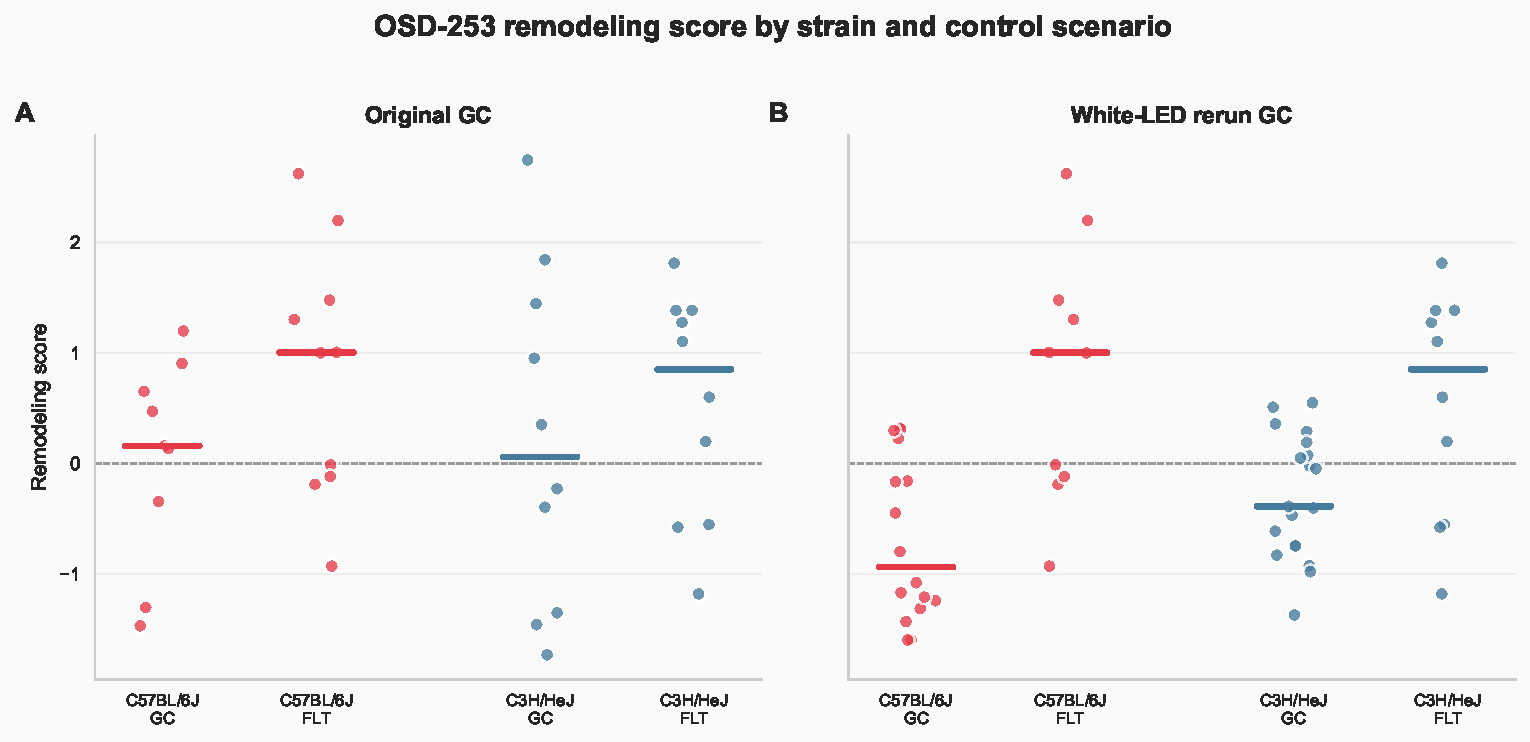
\includegraphics[width=\textwidth]{fig5_osd253_strain_points.pdf}
\caption{\textbf{OSD-253 remodeling score by strain and control scenario.} Points are individual mice, and colored bars show medians. The remodeling score is lower in C3H/HeJ at the point-estimate level, but the program remains positive under the white-LED rerun control scenario.}
\label{fig:osd253}
\end{figure}

TLR4/innate signaling tracks the remodeling score strongly, especially in OSD-253, and remains a plausible contextual axis. The strain comparison favors a TLR4-associated but broader remodeling program. Other mechanisms, including TGF-beta/EMT, adhesion, proteolysis, S1P signaling, macrophage context, and preservation stress, remain plausible contributors or covariates.

\subsection{WGCNA provides structural annotation of the remodeling program}

The WGCNA module layer annotates the remodeling program. A prior WGCNA analysis identified grey60 as a 48-gene ECM/cell-migration module with an ISS-T-specific eigengene pattern and hub structure involving genes such as \gene{Tril}, \gene{Itga9}, \gene{Fbn1}, \gene{S1pr3}, \gene{Cdh11}, \gene{Adam12}, and \gene{Mmp14}. That hub composition is consistent with the mechanism-axis result.

Follow-up overlap analyses place grey60 inside a broader multi-module response. The 11 ISS-T-Young LIONESS factorial edge-rewiring candidates distributed across purple, turquoise, yellow, black, brown, and one off-panel feature. Silent-shifter candidates enriched midnightblue in ISS-T-Young (11/185; $q=0.0031$) and purple in ISS-T-Old (13/171; $q=0.030$). Module eigengene contrasts showed an ISS-T-specific pattern in grey60, royalblue, salmon, and pink. WGCNA therefore supports structural annotation of a multi-module remodeling response, with grey60 as the most biologically interpretable ECM/cell-migration module.

\subsection{LIONESS/node2vec prioritizes candidate local-neighborhood contributors}

The exploratory LIONESS/node2vec ranking asked which genes show ISS-T-specific local network-neighborhood movement, stronger ISS-T node-strength effects than LAR, and support from OSD-513. In the 2,500-gene production run, the top composite genes included \gene{Rbm3}, \gene{Cyp4a14}, \gene{Bhmt}, \gene{Per2}, \gene{Hmgcr}, \gene{Sim2}, \gene{Hacl1}, \gene{Plin5}, \gene{Gpt}, \gene{Prodh}, and \gene{Ugt1a10}. In the 5,000-gene sensitivity run, high-ranking genes included \gene{Rbm3}, \gene{Bhmt}, \gene{Kank3}, \gene{Ugt1a10}, \gene{Ptpn1}, \gene{Serpinb8}, \gene{Cd200}, \gene{Per2}, and \gene{Cyp4a14}.

These genes are candidate local-neighborhood contributors to the pathway-level program. Top-k mechanism enrichment was weak after FDR correction (Figure~\ref{fig:genesens}). In the 2,500-gene production run, the strongest top-k findings were broad tubular transport at top 250 (2/4 genes; fold enrichment 5.0; raw $p=0.052$; $q=0.384$) and preservation stress at top 250 (3/10; fold enrichment 3.0; raw $p=0.070$; $q=0.384$). Ranked-list enrichment suggested broad tubular transport enrichment in the composite score (raw $p=0.0085$, $q=0.076$). In the 5,000-gene sensitivity run, the best ranked-list signals were preservation stress, broad tubular transport, and oxidative stress, all with $q=0.130$ or weaker.

\begin{figure}[H]
\centering
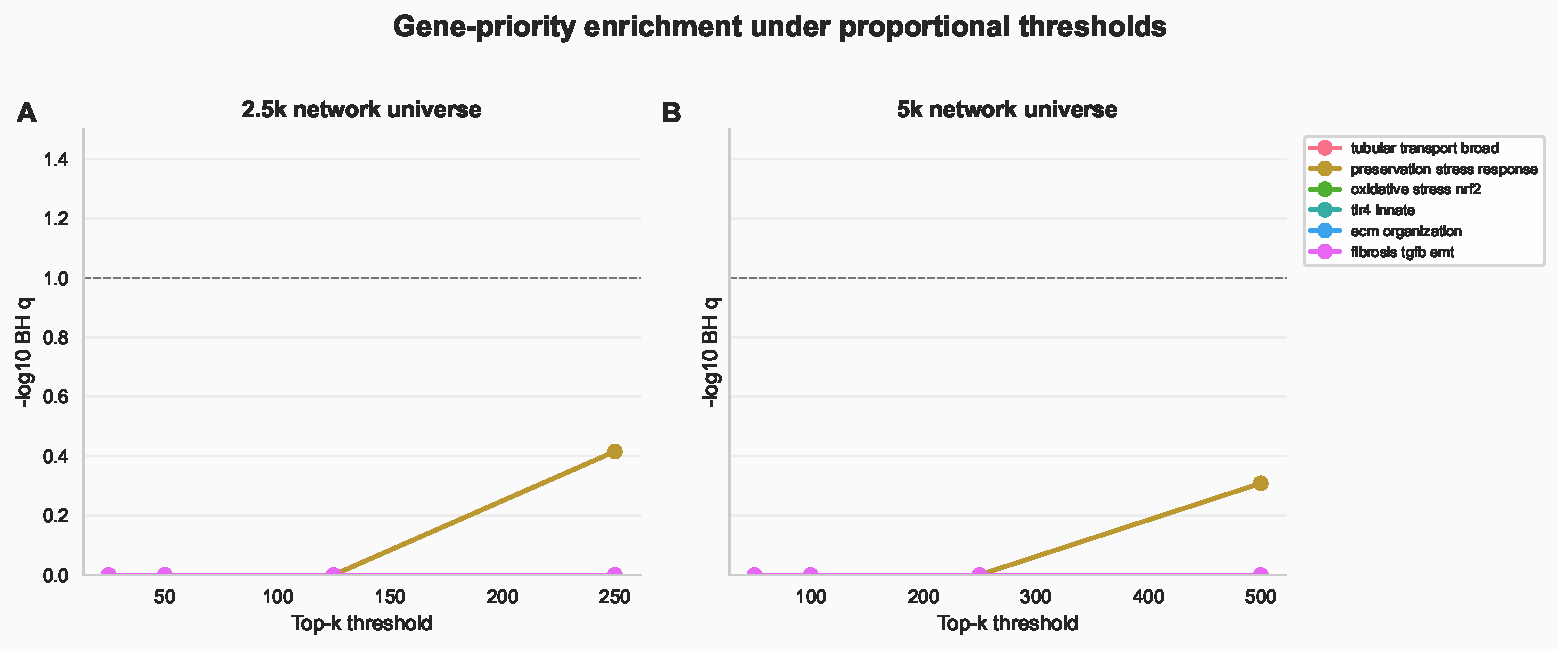
\includegraphics[width=\textwidth]{fig7_gene_priority_sensitivity.pdf}
\caption{\textbf{Top-k sensitivity for LIONESS/node2vec gene prioritization.} The gene-priority layer nominates candidate local-neighborhood contributors. The most consistent weak signals involve broad tubular transport, preservation stress, and oxidative/NRF2 context, while FDR support remains below the pathway/module-scale evidence.}
\label{fig:genesens}
\end{figure}

Node2vec and LIONESS add a gene-prioritization layer: they rank genes whose local network context moves with the ISS-T remodeling program. This layer is useful for follow-up target selection and gene-level annotation of the pathway/module result.

\subsection{External aging-axis projection favors remodeling over aging mimicry}

Projection onto the Tabula Muris Senis kidney aging axis separated the ISS-T remodeling program from simple aging mimicry. ISS-T was essentially orthogonal to the external aging vector ($\beta=-0.0027$, cosine $=-0.0187$). LAR had a small positive projection ($\beta=0.0162$, cosine $=0.175$), but the magnitude was small and the residual component remained dominant. The ISS-T signal is therefore best described as recurrent remodeling and transport biology rather than accelerated kidney aging.

\subsection{Claim hierarchy emerging from the full analysis}

The final claim hierarchy is:
\begin{enumerate}
  \item RRRM-2 cannot resolve the original age-rewiring contrast at primary module/pathway scale.
  \item RRRM-2 ISS-T, not LAR, aligns with an independent OSD-513 kidney flight vector.
  \item The aligned direction is a matrix-high / DCT-low tubulointerstitial state.
  \item OSD-253 suggests TLR4/innate association, while the C3H/HeJ comparison favors a broader remodeling program rather than strict TLR4 requirement.
  \item WGCNA, LIONESS, and node2vec provide annotation and exploratory gene prioritization below the cross-cohort pathway/module result.
\end{enumerate}

% =====================================================================
\section{Discussion}

\subsection{Principal finding}

The principal finding is an ISS-T-aligned kidney remodeling axis that recurs across OSDR cohorts. RRRM-2 defines arm-specific flight directions, and the ISS-T direction recurs in OSD-513. That recurrent direction is biologically coherent: a matrix-high / DCT-low tubulointerstitial state with mechanism-score support for innate immune context, adhesion/proteolysis, S1P signaling, and macrophage/inflammatory programs.

The analysis separates structural annotation from cross-cohort recurrence. WGCNA identifies ECM/cell-migration module structure in ISS-T. Cross-OSDR contrast analysis shows that the ISS-T direction recurs in an independent kidney flight cohort. Mechanism scoring places the recurring direction in biologically plausible fibrosis/transport/innate-immune machinery. OSD-253 places TLR4/innate biology as an associated context within a broader remodeling program.

\subsection{Biological interpretation: recurrent remodeling}

The strongest evidence is coordinated movement along a recurring pathway/module direction. The biological term used here is remodeling: a coordinated matrix and tubular-transport response that appears in RRRM-2 ISS-T and OSD-513. The state-space analysis makes that response visible as higher ECM/adhesion/proteolysis and lower DCT/NCC-WNK transport, with DCT kept in its native biological direction. The network methods remain useful because they localize candidate genes and modules within that response, but the central result is the cross-cohort pathway direction.

\subsection{Relationship to renal fibrosis and tubular transport literature}

The ECM/fibrosis-positive and DCT/NCC-WNK-negative axis is biologically plausible. Renal fibrosis involves extracellular matrix deposition, fibroblast activation, inflammatory signaling, TGF-beta pathways, cell adhesion, matrix proteolysis, and altered epithelial state \citep{liu2011fibrosis,natneph2024fibrosis,jci2024fibrosis,chavula2022cadherin}. TLR4 and innate immune signaling can promote inflammatory and fibrotic renal injury, and OSD-253 places that biology near the remodeling score without reducing the program to a single receptor axis \citep{souza2015tlr4,carpenter2009tril,carpenter2011tril,wochal2014tril}. S1P/S1PR3 biology is also relevant because sphingolipid signaling can influence vascular, inflammatory, and fibrotic responses \citep{s1p2017,s1p2020,s1p2009}. Distal convoluted tubule transport is regulated by NCC and the WNK-SPAK/OSR1 pathway, and changes in this axis can reflect altered electrolyte handling and tubular adaptation \citep{castaneda2024dct,ge2016wnk}.

The important caveat is that transcriptomic pathway direction is molecular evidence for fibrotic and transport remodeling, not histology or physiology. It nominates a direction to test with collagen staining, tubular injury markers, urine/serum chemistry, segment-specific NCC/WNK markers, and perturbation studies.

\subsection{Interpretation of OSD-253}

OSD-253 asks a mechanism-context question: if the ISS-T-aligned remodeling axis is tied to TLR4/innate signaling, does it attenuate in C3H/HeJ? The remodeling score is lower in C3H/HeJ at the point-estimate level, with strain-delta confidence intervals crossing zero. ECM, fibrosis/TGF-beta, adhesion, and proteolysis scores remain positive in C3H/HeJ under the white-LED rerun scenario. OSD-253 therefore supports a distributed remodeling model in which TLR4/innate biology is associated with the axis while other ECM, adhesion, proteolysis, and transport programs remain active.

The TLR4/innate score strongly tracks the remodeling score across OSD-253 samples, and TRIL/TLR-related hub structure in the WGCNA ECM module remains biologically interesting. The revised interpretation is that TLR4/innate biology is a candidate context or amplifier within a broader ECM/transport remodeling response.

\subsection{What the LIONESS/node2vec layer adds}

The LIONESS/node2vec layer answers a secondary question: which genes may have local network neighborhoods that move with the recurrent remodeling program? The top-ranked genes include stress-response, metabolic, circadian, transport, and signaling candidates. This layer can guide follow-up exploration, gene-set annotation, and figure supplements. The pathway/module result remains the claim anchor; the network-neighborhood ranking supplies candidate genes for interpretation and validation.

\subsection{Limitations}

Several limitations are central. First, RRRM-2 has only $n=5$ per factorial cell, which limits high-dimensional interaction estimation. Second, ISS-T and LAR differ in flight state, return/recovery timing, and collection context; their contrast should not be interpreted as a pure biological recovery experiment. Third, external OSDR cohorts differ in sex, strain, mission, duration, sequencing, and metadata. Cross-cohort agreement at pathway-vector level is meaningful, while raw expression pooling would be inappropriate. Fourth, OSD-253 has two imperfect control definitions, and both must remain visible in the manuscript. Fifth, the mechanism signatures are curated and relatively small; coverage and de-overlap tables help audit them but cannot eliminate annotation bias. Sixth, the bootstrap resamples samples under fixed preprocessing, deconvolution, residualization, gene-set, and pathway-selection choices; it does not propagate all pipeline-level uncertainty. Seventh, Tabula Muris Senis provides an external aging reference with a larger age span than RRRM-2, so weak projection argues against simple aging mimicry but cannot rule out subtler age interactions.

\subsection{Future work}

The most direct experimental follow-up is to test the remodeling axis in tissue. Histology for collagen deposition, tubular injury, immune infiltration, and distal-nephron markers would distinguish transcriptomic remodeling from structural fibrosis. Segment-specific assays could test whether DCT/NCC-WNK suppression corresponds to altered NCC abundance or phosphorylation. Mechanistically, TLR4-impaired and TLR4-intact comparisons should be paired with additional perturbations or markers because OSD-253 points to a broader remodeling response. Computationally, the next step is to keep the claim hierarchy intact, expand external cohorts when metadata supports it, and use network-neighborhood rankings as hypothesis generation for targeted validation.

% =====================================================================
\section{Conclusion}

RRRM-2's strongest estimable claim is an ISS-T-aligned kidney remodeling axis that recurs in OSD-513. The axis is best described as a matrix-high / DCT-low tubulointerstitial state and is embedded in TLR4/innate, adhesion/proteolysis, S1P, macrophage/inflammation, and sample-context biology. OSD-253 places TLR4/innate signaling as an associated context within a broader remodeling program. WGCNA and LIONESS/node2vec provide annotation and exploratory prioritization layers below the cross-cohort pathway/module claim.

\section*{Author contributions}
I.S. designed and implemented the analytical framework, conducted the contrast-vector, cross-OSDR, mechanism-axis, WGCNA-context, LIONESS/node2vec, and sensitivity analyses, generated the figures, drafted the manuscript, and maintained the source code, tests, and run artifacts. Authorship and collaboration structure will be revised with mentor and collaborator input.

\section*{Competing interests}
The author declares no competing interests.

\section*{Data and code availability}
NASA Open Science Data Repository accessions: OSD-771 (RRRM-2), OSD-513, and OSD-253. Tabula Muris Senis kidney was used as the external aging reference. Pipeline source, configuration files, run manifests, tests, figures, and manuscript drafts are version-controlled in the project repository.

\begin{itemize}
  \item Main v4 production run: \code{run\_20260519\_000547\_2500g}.
  \item Cross-OSDR permutation sensitivity run: \code{run\_20260519\_cosine\_perm\_null}.
  \item Primary mechanism-axis outputs: \path{data/results/run_20260519_000547_2500g/contrast_vectors/mechanism_axis}.
  \item Tubulointerstitial state-space outputs: \path{data/results/run_20260519_000547_2500g/contrast_vectors/mechanism_axis/tubulointerstitial_state}.
  \item 5,000-gene sensitivity run: \code{run\_20260519\_5000g\_sensitivity\_3seed}.
  \item Figure-generation script: \path{scripts/plot_manuscript_v4_figures.py}.
  \item Pipeline entry point: \path{venv/bin/python -m src.run_all_phases --updated-pipeline}.
\end{itemize}

% =====================================================================
\begin{thebibliography}{99}\small

\bibitem{afshinnekoo2020fundamental} Afshinnekoo E, Scott RT, MacKay MJ, et al. Fundamental biological features of spaceflight: advancing the field to enable deep-space exploration. \emph{Cell}. 2020;183:1162--1184. doi:10.1016/j.cell.2020.10.050.

\bibitem{benjamini1995controlling} Benjamini Y, Hochberg Y. Controlling the false discovery rate: a practical and powerful approach to multiple testing. \emph{Journal of the Royal Statistical Society Series B}. 1995;57:289--300.

\bibitem{carpenter2009tril} Carpenter S, Carlson T, Dellacasagrande J, et al. TRIL, a functional component of the TLR4 signaling complex, highly expressed in brain. \emph{Journal of Immunology}. 2009. doi:10.4049/jimmunol.0901518.

\bibitem{carpenter2011tril} Carpenter S, Wochal P, Dunne A, O'Neill LAJ. Toll-like receptor 3 and Toll-like receptor 4 accessory protein TRIL. \emph{Journal of Biological Chemistry}. 2011. doi:10.1074/jbc.M111.255893.

\bibitem{castaneda2024dct} Castaneda-Bueno M, et al. The distal convoluted tubule and sodium chloride cotransporter regulation in kidney physiology. \emph{Pfluegers Archiv}. 2024. doi:10.1007/s00424-024-03029-5.

\bibitem{chavula2022cadherin} Chavula T, et al. Cadherin-11 and its role in tissue fibrosis. \emph{Cells Tissues Organs}. 2022;212:293--309. doi:10.1159/000525359.

\bibitem{chouker2025impact} Chouker A, Gallo A, et al. Impact of spaceflight on endocrine, metabolic and kidney function: current evidence, open issues, and potential countermeasures. \emph{BMC Biology}. 2025. doi:10.1186/s12915-025-02471-w.

\bibitem{cockett1962astronautical} Cockett ATK, Beehler CC, Roberts JE. Astronautical urolithiasis: a potential hazard during prolonged weightlessness in space travel. \emph{Journal of Urology}. 1962;88:542--544.

\bibitem{daSilveira2020comprehensive} da Silveira WA, Fazelinia H, Rosenthal SB, et al. Comprehensive multi-omics analysis reveals mitochondrial stress as a central biological hub for spaceflight impact. \emph{Cell}. 2020;183:1185--1201. doi:10.1016/j.cell.2020.10.005.

\bibitem{finch2025strain} Finch RH, Vitry G, Siew K, Walsh SB, Beheshti A, Hardiman G, da Silveira WA. Spaceflight causes strain-dependent gene expression changes in the kidneys of mice. \emph{npj Microgravity}. 2025. doi:10.1038/s41526-025-00465-0.

\bibitem{galazka2020rnaseq} Galazka JM, et al. RNAseq analysis of rodent spaceflight experiments is confounded by sample collection techniques. \emph{iScience}. 2020;23:101733. doi:10.1016/j.isci.2020.101733.

\bibitem{ge2016wnk} Ge Y, et al. WNK pathway genes and renal electrolyte transport biology. \emph{Gene}. 2016. doi:10.1016/j.gene.2016.07.033.

\bibitem{grover2016node2vec} Grover A, Leskovec J. node2vec: scalable feature learning for networks. \emph{Proceedings of the 22nd ACM SIGKDD International Conference on Knowledge Discovery and Data Mining}. 2016. doi:10.1145/2939672.2939754.

\bibitem{jci2024fibrosis} Dumoulin B, Susztak K. Fibrosis uncovered: ADAMTS12 cuts to the core of extracellular matrix drama. \emph{Journal of Clinical Investigation}. 2024;134:e183115. doi:10.1172/JCI183115.

\bibitem{kuijjer2019estimating} Kuijjer ML, Tung MG, Yuan G, Quackenbush J, Glass K. Estimating sample-specific regulatory networks. \emph{iScience}. 2019;14:226--240. doi:10.1016/j.isci.2019.03.021.

\bibitem{langfelder2008wgcna} Langfelder P, Horvath S. WGCNA: an R package for weighted correlation network analysis. \emph{BMC Bioinformatics}. 2008;9:559. doi:10.1186/1471-2105-9-559.

\bibitem{langfelder2011preservation} Langfelder P, Luo R, Oldham MC, Horvath S. Is my network module preserved and reproducible? \emph{PLoS Computational Biology}. 2011;7:e1001057. doi:10.1371/journal.pcbi.1001057.

\bibitem{liu2011fibrosis} Liu Y. Cellular and molecular mechanisms of renal fibrosis. \emph{Nature Reviews Nephrology}. 2011;7:684--696. doi:10.1038/nrneph.2011.149.

\bibitem{love2014deseq2} Love MI, Huber W, Anders S. Moderated estimation of fold change and dispersion for RNA-seq data with DESeq2. \emph{Genome Biology}. 2014;15:550. doi:10.1186/s13059-014-0550-8.

\bibitem{natneph2024fibrosis} Allison SJ. ECM remodelling by ADAMTS12 in fibrosis. \emph{Nature Reviews Nephrology}. 2024;20:770. doi:10.1038/s41581-024-00905-2.

\bibitem{pietrzyk2007renal} Pietrzyk RA, Jones JA, Sams CF, Whitson PA. Renal stone formation among astronauts. \emph{Aviation, Space, and Environmental Medicine}. 2007;78:A9--A13.

\bibitem{preserve2016} Ray S, et al. Preservation of multiple mammalian tissues to maximize science return from ground based and spaceflight experiments. \emph{PLOS ONE}. 2016. doi:10.1371/journal.pone.0167391.

\bibitem{ray2019genelab} Ray S, Gebre S, Fogle H, et al. GeneLab: omics database for spaceflight experiments. \emph{Bioinformatics}. 2019;35:1753--1759.

\bibitem{ritchie2015limma} Ritchie ME, Phipson B, Wu D, et al. limma powers differential expression analyses for RNA-sequencing and microarray studies. \emph{Nucleic Acids Research}. 2015;43:e47. doi:10.1093/nar/gkv007.

\bibitem{robinson2010edger} Robinson MD, McCarthy DJ, Smyth GK. edgeR: a Bioconductor package for differential expression analysis of digital gene expression data. \emph{Bioinformatics}. 2010;26:139--140. doi:10.1093/bioinformatics/btp616.

\bibitem{s1p2009} Hla T, et al. Sphingosine-1-phosphate signaling in physiology and disease. \emph{Medecine/Sciences}. 2009. doi:10.1051/medsci/2009252161.

\bibitem{s1p2017} Du C, Ren Y, Yao F, et al. Sphingosine kinase 1 protects renal tubular epithelial cells from renal fibrosis via induction of autophagy. \emph{International Journal of Biochemistry and Cell Biology}. 2017;90:17--28. doi:10.1016/j.biocel.2017.07.011.

\bibitem{s1p2020} Donati C, Cencetti F, Bernacchioni C, Vannuzzi V, Bruni P. Role of sphingosine 1-phosphate signalling in tissue fibrosis. \emph{Cellular Signalling}. 2021;78:109861. doi:10.1016/j.cellsig.2020.109861.

\bibitem{siew2024cosmic} Siew K, Nestler KA, Nelson C, et al. Cosmic kidney disease: an integrated pan-omic, physiological and morphological study into spaceflight-induced renal dysfunction. \emph{Nature Communications}. 2024;15:4923. doi:10.1038/s41467-024-49212-1.

\bibitem{smith2014men} Smith SM, Heer M, Shackelford LC, Sibonga JD, Spatz J, Pietrzyk RA, Hudson EK, Zwart SR. Men and women in space: bone loss and kidney stone risk after long-duration spaceflight. \emph{Journal of Bone and Mineral Research}. 2014;29:1639--1645. doi:10.1002/jbmr.2185.

\bibitem{soma2024} Overbey EG, et al. The Space Omics and Medical Atlas across orbits. \emph{Nature}. 2024. doi:10.1038/s41586-024-07639-y.

\bibitem{souza2015tlr4} Souza ACP, et al. TLR4 mutant mice are protected from renal fibrosis and chronic kidney disease progression. \emph{Physiological Reports}. 2015. doi:10.14814/phy2.12558.

\bibitem{tabula2020} The Tabula Muris Consortium. A single-cell transcriptomic atlas characterizes ageing tissues in the mouse. \emph{Nature}. 2020;583:590--595. doi:10.1038/s41586-020-2496-1.

\bibitem{wochal2014tril} Wochal P, et al. TRIL is involved in cytokine production following Toll-like receptor activation. \emph{Journal of Immunology}. 2014. doi:10.4049/jimmunol.1302392.

\end{thebibliography}

\vspace{1em}
\begin{center}
\rule{0.4\textwidth}{0.4pt}
\end{center}
\vspace{0.3em}
\noindent\textit{Draft v4 prepared May 2026. Reference metadata should still be curated against a journal style file before submission, but the current draft anchors the main biological and statistical claims to the relevant scholarly literature.}

\end{document}
